\newcounter{case}
\newcommand\case{\stepcounter{case}\arabic{case}}
\chapter{SPECIFIC REQUIREMENTS}
\label{ch:specificRequirements}%
% The \label{...}% enables to remove the small indentation that is generated, always leave the % symbol.
\section{External Interface Requirements}
\label{sec:externalInterfaceRequirements}
\subsection{User Interfaces}
\label{subsec:userInterfaces}
The following mockups are presented here just to show an idea of the application
that will be in use by the Drivers and the one available to the CPOs. In Figure \ref{fig:map} and \ref{fig:book} are shown some of the functionalities available to the eMSP, such as the Map and the charging station availability. On the other hand, by figure \ref{fig:CPMS} it's possible to see the list of the CPO's managed charging stations, as well as the eMSP association functionality. The complete list of mockups (mobile app for eMSP and application for CMPS) will be available in the design document.
\begin{figure}[H]
    \begin{minipage}[t]{.35\textwidth} % not "0.5\textwidth"
    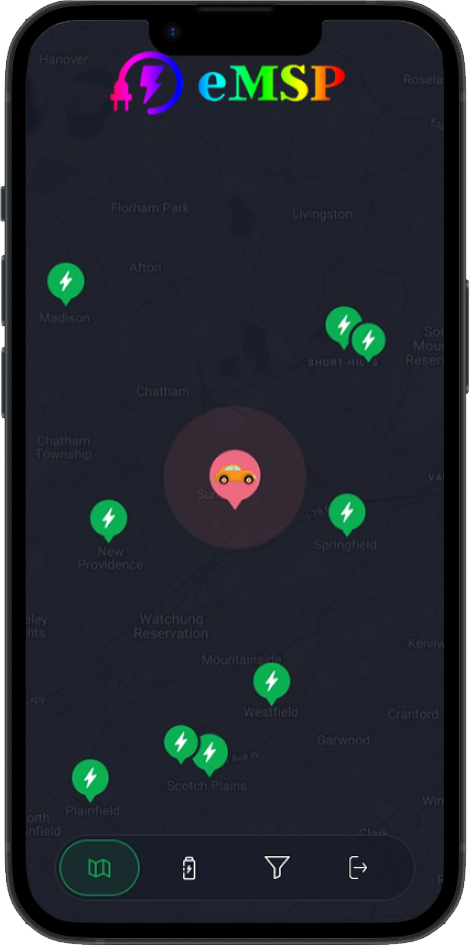
\includegraphics[width=\textwidth]{Mock/map}
    \caption{Map Mockup}
    \label{fig:map}
\end{minipage}
\hfill
\begin{minipage}[t]{.35\textwidth}
    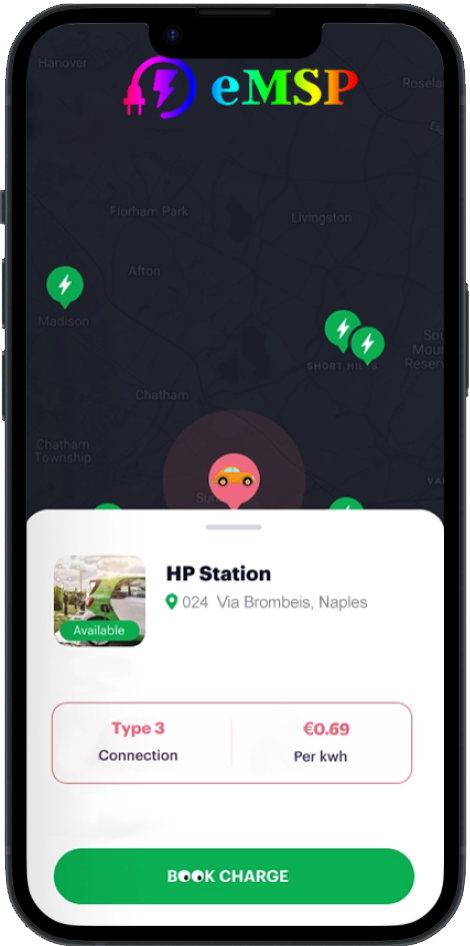
\includegraphics[width=\textwidth]{Mock/book}
    \caption{Booking Mockup}
    \label{fig:book}
\end{minipage}
\end{figure}
\begin{figure}[H]
            \begin{center}
            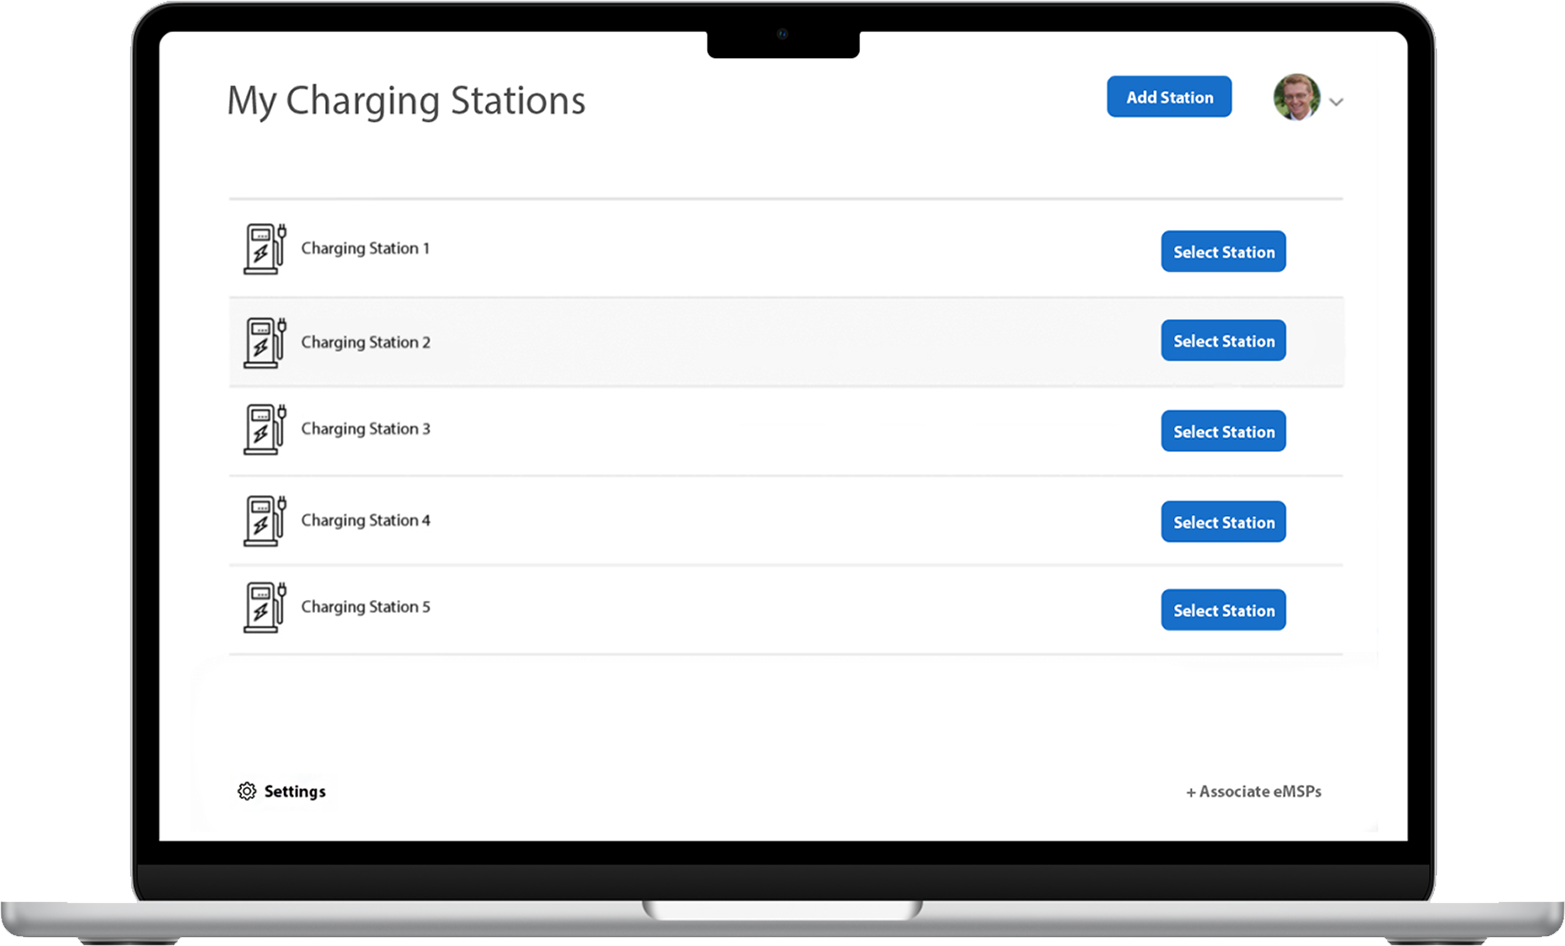
\includegraphics[
                width=\textwidth,
                height=\textheight,
                keepaspectratio]{Mock/CPMS}
            \caption{CPMS Mockup}
            \label{fig:CPMS}
            \end{center}
        \end{figure}
\subsection{Hardware Interfaces}
\label{subsec:hardwareInterfaces}
\begin{itemize}
    \item \textbf{Vehicle Interface}: Since the system requires to access info from the Driver's vehicle, such as the battery level, the location or the navigation route, it is necessary to establish a connection between the two of them. This should be done by the Driver through his device in order to let him receive suggestions.
    \item \textbf{Charging Station Interface}: In order to add and manage charging stations to the system there must be an interface between the two of them that permits the exchange of data through a standard protocol.
    \item \textbf{Charging Socket Interface}: In order to manage the charging process, check both its status and the connection between the vehicle and its connected socket, there must be an interface between the system and charging sockets that permits the exchange of data through a standard protocol.
    %\item \textbf{eMSP}: \\
     %   In order to install and utilize the system the Driver needs to have a mobile device with an internet connection. It should be able to run the application, which requires rendering of maps. Furthermore, it should be able to connect with his vehicle. The connection between the mobile device and the vehicle should allow to extrapolate data, such as battery status and navigation routes, from the vehicle and send it to eMSP through the mobile device. 
    %\item \textbf{CPMS}: \\
     %   In order to install and utilize the system, the CPO should have access to a machine capable of hosting the CPMS Server and another device, such as any computer, capable of elaborating and making requests to the CPMS server. The server machine is required to have a stable internet connection in order be able to talk with eMSPs subsystems and receive multiple requests from them.
\end{itemize}
\subsection{Software Interfaces}
\label{subsec:softwareInterfaces}
The CPMS and eMSP communicate with each other through a uniform API, in order to exchange information. In particular, the CPMS has to update all the eMSPs that are associated with him about socket availability and stations' charging prices; meanwhile, the eMSP has to communicate with the CPMS in order to let the Driver perform operations for recharging his vehicle and create/delete bookings. In order to do so, all the CPMSs and the eMSPs should have the same external interface protocol and attain themselves to this standard.
\subsection{Communication Interfaces}
\label{subsec:communicationInterfaces}
The systems, both the eMSP and the CPMS, communicate with external APIs in order to provide all the different functions described in section \ref{sec:productFunctions}.
\begin{itemize}
    %\item \textbf{Charging station} - The CPMS communicates with charging stations and charging socket in order to receive data about physical events such as vehicle connected or charge finished and perform operations, like starting a charge. 
    \item \textbf{Payment API} - In order for the Driver to pay the relative CPO for the given charging service, the eMSP uses an external API that allows and manages payments.
    \item \textbf{Maps API} - In order to show the Driver where all the charging stations are located, the eMSP uses an external API that provides up-to-date maps.
    \item \textbf{Calendar API} - In order to generate suggestions for the Driver, the eMSP application can check the calendar events through this API.
    \item \textbf{eMall API} - The eMall system provides the following APIs in order to let the eMSP and the CPMS communicate with it:
        \begin{itemize}
            \item \textbf{Confirming credentials} - The CPO credentials used to access the CPMS are authenticated on the eMall system.
            \item \textbf{eMSP List} - The CPMS retrieves a list of all the existing eMSPs from the eMall system, in order to show them to the CPO.
        \end{itemize}
   \item \textbf{DSO API} - The CPMS uses an external uniform API to retrieve the DSOs prices and energy capacity, in order to choose which one to get energy from. 
   %\item \textbf{Charging Station modules} - The CPMS needs to be able to communicate with the charging station in order to detect whether a new one has been managed by the CPO.     
\end{itemize}
\label{subsec:sequenceDiagrams}
\section{Functional Requirements}
\label{sec:functionalRequirements}
\subsection{Use Case Diagrams}
\begin{enumerate}
    \item \textbf{Unregistered Driver}
        \begin{figure}[H]
            \begin{center}
            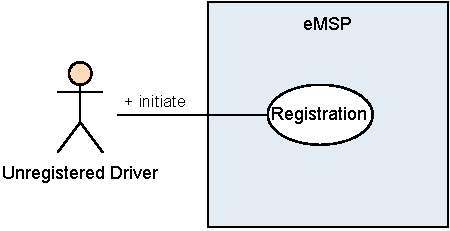
\includegraphics[
                width=0.6\textwidth,
                height=\textheight,
                keepaspectratio]{UseCaseDia/UnregisteredDriver}
            \caption{Use case diagram for an Unregistered Driver}
            \label{fig:UnregisteredDriver}
            \end{center}
        \end{figure}
        \newpage
    \item \textbf{Driver}
        \begin{figure}[H]
            \begin{center}
            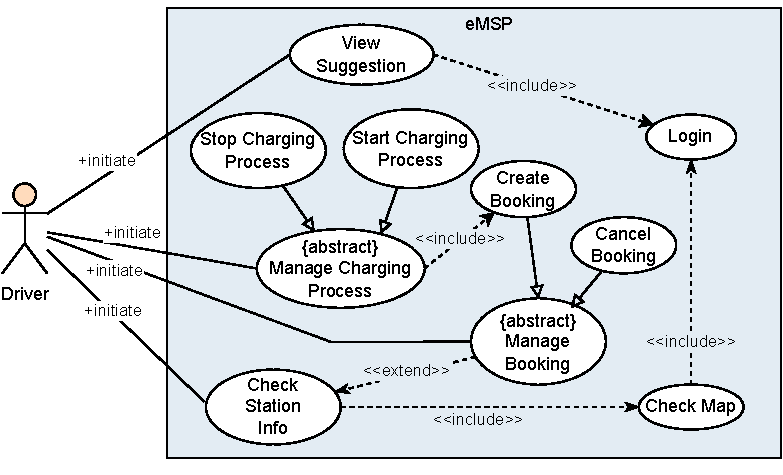
\includegraphics[
                width=\textwidth,
                height=\textheight,
                keepaspectratio]{UseCaseDia/Driver}
            \caption{Use case diagram for a Driver}
            \label{fig:UnregisteredDriver}
            \end{center}
        \end{figure}
    \item \textbf{CPO}
        \begin{figure}[H]
            \begin{center}
            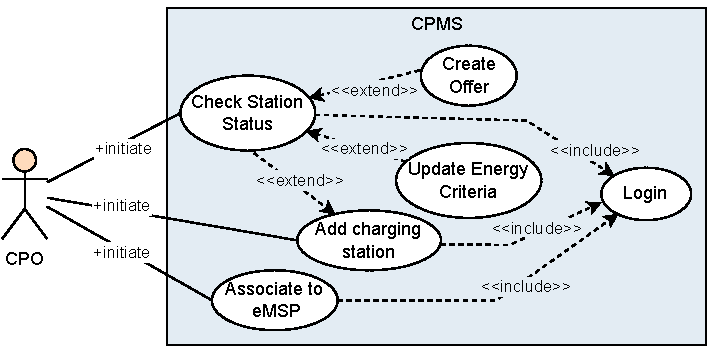
\includegraphics[
                width=\textwidth,
                height=\textheight,
                keepaspectratio]{UseCaseDia/CPO}
            \caption{Use case diagram for a CPO}
            \label{fig:UnregisteredDriver}
            \end{center}
        \end{figure}
\end{enumerate}
\label{subsec:useCaseDiagrams}
\newpage
\subsection{Use Cases}
\label{subsec:useCases}
\textbf{Note}: In the following use cases we assume no internet connection failures.
% belliximo template per gli use cases by Andrea BIBA
% se si usa longtable gli elenchi escono con un padding orribile
% quindi meglio tenere tabular
\begin{enumerate}
    \item \textbf{Driver Registration} 
    \begin{table}[H]
        \centering
    \begin{tabular}{| >{\columncolor{bluepoli!15}}p{0.30\linewidth} |p{0.7\linewidth} |}
        \hline
        \rowcolor{bluepoli!40}
        \textbf{Use Case \case} & \textbf{Driver Registration} \T\B \\
        \hline 
        \hline
        \textbf{Actor(s)} & Unregistered Driver \T\B\\
        \hline
        \textbf{Entry Condition} & The driver does not have an account and is on the initial view of the eMSP \T\B\\ 
        \hline
        \textbf{Event Flow} &     
        \begin{enumerate}
            \item The Unregistered Driver press the "Register" button
            \item The Unregistered Driver enters name, birth, date, email address and password
            \item The Unregistered Driver submits the compiled form
            \item The eMSP processes the request and shows a success message
        \end{enumerate}\T\B\\
        \hline
        \textbf{Exit Condition} & An account is created \T\B\\
        \hline
        \textbf{Exception} & The driver does not enter all mandatory data. The exception is notified to the Driver. \T\B\\
        \hline
    \end{tabular}
    \end{table}
    \item \textbf{ Driver Login} 
    \begin{table}[H]
        \centering
    \begin{tabular}{| >{\columncolor{bluepoli!15}}p{0.30\linewidth} |p{0.7\linewidth} |}
        \hline
        \rowcolor{bluepoli!40}
        \textbf{Use Case \case} & \textbf{Driver Login} \T\B \\
        \hline 
        \hline
        \textbf{Actor(s)} & Registered Driver \T\B\\
        \hline
        \textbf{Entry Condition} & Driver is not logged in and on the eMSP main page \T\B\\ 
        \hline
        \textbf{Event Flow} &     
        \begin{enumerate}
            \item The Driver press the "Login" button
            \item The Driver submits his credentials such as email and password 
            \item The eMSP validates his credentials and shows a success message
        \end{enumerate}\T\B\\
        \hline
        \textbf{Exit Condition} & The driver is logged into the eMSP\T\B\\
        \hline
        \textbf{Exception} & 
         Users enters invalid credentials. The exception is notified to the Driver. \T\B\\
        \hline
    \end{tabular}
    \end{table}
    \newpage
    \item \textbf{ Driver checks map}
    \begin{table}[H]
        \centering
    \begin{tabular}{| >{\columncolor{bluepoli!15}}p{0.30\linewidth} |p{0.7\linewidth} |}
        \hline
        \rowcolor{bluepoli!40}
        \textbf{Use Case \case} & \textbf{Driver checks map} \T\B \\
        \hline 
        \hline
        \textbf{Actor(s)} & Driver \T\B\\
        \hline
        \textbf{Entry Condition} & Driver is logged in \T\B\\ 
        \hline
        \textbf{Event Flow} &     
        \begin{enumerate}
            \item The Driver opens the eMSP application and gets on the Map view
            \item (opt) The Driver moves to the area in which he wants to see all the charging stations
            \item (opt) The Driver selects the charging type filter to apply to the map
            \item The eMSP processes the request and returns the charging stations on the map that match the filters in that area
        \end{enumerate}\T\B\\
        \hline
        \textbf{Exit Condition} & All the stations are shown to the Driver\T\B\\
        \hline
        \textbf{Exception} & There are no available stations matching the filter in the requested area. The system sends a notification to warn the Driver. \T\B\\
        \hline
    \end{tabular}
    \end{table}
    \item \textbf{ Driver checks charging station info}
    \begin{table}[H]
        \centering
    \begin{tabular}{| >{\columncolor{bluepoli!15}}p{0.30\linewidth} |p{0.7\linewidth} |}
        \hline
        \rowcolor{bluepoli!40}
        \textbf{Use Case \case} & \textbf{Driver checks charging station info} \T\B \\
        \hline 
        \hline
        \textbf{Actor(s)} & Driver \T\B\\
        \hline
        \textbf{Entry Condition} & Driver is on the map page \T\B\\ 
        \hline
        \textbf{Event Flow} &     
        \begin{enumerate}
            \item The Driver clicks on one of the shown charging stations
            \item The eMSP processes the request and returns the info of that charging station, such as its charging prices for each charging type, the address and the availability
            \item The Driver sees the received info
        \end{enumerate}\T\B\\
        \hline
        \textbf{Exit Condition} & Info of the stations are correctly shown to the Driver. \T\B\\
        \hline
        \textbf{Exception} & None \T\B\\
        \hline
    \end{tabular}
    \end{table}
    \newpage
    \item \textbf{Book a charge}
    \begin{table}[H]
        \centering
    \begin{tabular}{| >{\columncolor{bluepoli!15}}p{0.30\linewidth} |p{0.7\linewidth} |}
        \hline
        \rowcolor{bluepoli!40}
        \textbf{Use Case \case} & \textbf{Book a charge} \T\B \\
        \hline 
        \hline
        \textbf{Actor(s)} & Driver \T\B\\
        \hline
        \textbf{Entry Condition} & Driver is checking the details of a station \T\B\\ 
        \hline
        \textbf{Event Flow} &     
        \begin{enumerate}
            \item The Driver clicks on the "Book charge" button
            \item The Driver selects the arrival time
            \item The Driver clicks on "Submit" and sends the request
            \item The eMSP notifies the user that he has successfully booked a charge and the ID of the charging socket
        \end{enumerate}\T\B\\
        \hline
        \textbf{Exit Condition} & The charge has been correctly booked \T\B\\
        \hline
        \textbf{Exception} & An exception is thrown to the eMSP by the CMPS. The exception message is notified to the Driver.\T\B\\
        \hline
    \end{tabular}
    \end{table}
    \item \textbf{Cancel a booked charge}
    \begin{table}[H]
        \centering
    \begin{tabular}{| >{\columncolor{bluepoli!15}}p{0.30\linewidth} |p{0.7\linewidth} |}
        \hline
        \rowcolor{bluepoli!40}
        \textbf{Use Case \case} & \textbf{Cancel a booked charge} \T\B \\
        \hline 
        \hline
        \textbf{Actor(s)} & Driver \T\B\\
        \hline
        \textbf{Entry Condition} & Driver has booked a charge\T\B\\ 
        \hline
        \textbf{Event Flow} &     
        \begin{enumerate}
            \item The Driver clicks on the Booked Charge button
            \item The Driver clicks on the "Delete Booking" button
            \item The eMSP notifies the user that the booked charge has been deleted
        \end{enumerate}\T\B\\
        \hline
        \textbf{Exit Condition} & The booked charge has been deleted \T\B\\
        \hline
        \textbf{Exception} & An exception is thrown to the eMSP by the CMPS. The exception message is notified to the Driver. \T\B\\
        \hline
    \end{tabular}
    \end{table}
    \newpage
    \item \textbf{Start charging process}
    \begin{table}[H]
        \centering
    \begin{tabular}{| >{\columncolor{bluepoli!15}}p{0.30\linewidth} |p{0.7\linewidth} |}
        \hline
        \rowcolor{bluepoli!40}
        \textbf{Use Case \case} & \textbf{Start charging process} \T\B \\
        \hline 
        \hline
        \textbf{Actor(s)} & Driver \T\B\\
        \hline
        \textbf{Entry Condition} & The driver has booked a charge and is arrived at the charging station \T\B\\ 
        \hline
        \textbf{Event Flow} &     
        \begin{enumerate}     
            \item The Driver clicks on the Booked Charge button and checks the socket ID he has booked   
            \item The Driver plugs his vehicle to the socket with the ID booked
            \item The Driver clicks on the "Start charge" button
            \item The eMSP processes the request and notifies the user that the charging process has been started
            \item The Driver sees the estimated time for the charge to end
        \end{enumerate}\T\B\\
        \hline
        \textbf{Exit Condition} & The charge is started \T\B\\
        \hline
        \textbf{Exceptions} & 
            The charge can't be started because the vehicle is not well connected with the socket. The exception is notified to the Driver. 
        \\
        \hline
    \end{tabular}
    \end{table}
    \item \textbf{Stop charging process}
    \begin{table}[H]
        \centering
    \begin{tabular}{| >{\columncolor{bluepoli!15}}p{0.30\linewidth} |p{0.7\linewidth} |}
        \hline
        \rowcolor{bluepoli!40}
        \textbf{Use Case \case} & \textbf{Stop charging process} \T\B \\
        \hline 
        \hline
        \textbf{Actor(s)} & Driver \T\B\\
        \hline
        \textbf{Entry Condition} & The driver is checking the detail of his charging process \T\B\\ 
        \hline
        \textbf{Event Flow} &     
        \begin{enumerate}
            \item The Driver clicks on the "Stop Charge" button
            \item The eMSP processes the request and notifies the user that the charging process has been stopped
            \item The eMSP notifies the user that the payment was successful
        \end{enumerate}\T\B\\
        \hline
        \textbf{Exit Condition} & The charge has been ended \T\B\\
        \hline
        \textbf{Exception} & The eMSP can't process the booking request due to an error while communicating with the CMPS. The exception is notified to the Driver. \T\B\\
        \hline
    \end{tabular}
    \end{table}
    \newpage
    \item \textbf{Suggestion Notification}
    \begin{table}[H]
        \centering
    \begin{tabular}{| >{\columncolor{bluepoli!15}}p{0.30\linewidth} |p{0.7\linewidth} |}
        \hline
        \rowcolor{bluepoli!40}
        \textbf{Use Case \case} & \textbf{Suggestion Notification} \T\B \\
        \hline 
        \hline
        \textbf{Actor(s)} & Driver \T\B\\
        \hline
        \textbf{Entry Condition} & The Driver has authorized the systems to read his data (calendar, vehicle's navigation routes, vehicle's location and vehicle's battery status) and receives a notification containing a suggested charging station where to charge his vehicle.  \T\B\\ 
        \hline
        \textbf{Event Flow} &
        (opt - Driver can ignore the notification)
        \begin{enumerate}
            \item The Driver clicks on the notification.
            \item The Driver is redirected to the station's info page.
        \end{enumerate}\T\B\\
        \hline
        \textbf{Exit Conditions} & 
        \begin{itemize}
            \item The Driver is on the station info page.
            \item The Driver ignores the notification.
        \end{itemize}  \T\B\\
        \hline
        \textbf{Exception} & None \T\B\\
        \hline
    \end{tabular}
    \end{table}
\item \textbf{CPO Login}
    \begin{table}[H]
        \centering
    \begin{tabular}{| >{\columncolor{bluepoli!15}}p{0.30\linewidth} |p{0.7\linewidth} |}
        \hline
        \rowcolor{bluepoli!40}
        \textbf{Use Case \case} & \textbf{CPO Login} \T\B \\
        \hline 
        \hline
        \textbf{Actor(s)} & CPO \T\B\\
        \hline
        \textbf{Entry Condition} & The CPO is not logged in and is on the initial view of the CPMS \T\B\\ 
        \hline
        \textbf{Event Flow} &     
        \begin{enumerate}
            \item The CPO presses the "Login" button.
            \item The CPO submits his credentials such as email and password.
            \item The CPMS validates his credentials and shows a success message.
        \end{enumerate}\T\B\\
        \hline
        \textbf{Exit Condition} & The CPO is logged into the CPMS and sees the list of his managed charging stations. \T\B\\
        \hline
        \textbf{Exception} & The CPO enters invalid credentials. The exception is notified to the CPO. \T\B\\
        \hline
        \end{tabular}
        \end{table}
        \newpage
\item \textbf{View managed charging station status}
    \begin{table}[H]
        \centering
    \begin{tabular}{| >{\columncolor{bluepoli!15}}p{0.30\linewidth} |p{0.7\linewidth} |}
        \hline
        \rowcolor{bluepoli!40}
        \textbf{Use Case \case} & \textbf{View managed charging station status} \T\B \\
        \hline 
        \hline
        \textbf{Actor(s)} & CPO \T\B\\
        \hline
        \textbf{Entry Condition} & The CPO is logged in \T\B\\ 
        \hline
        \textbf{Event Flow} &    
        \begin{enumerate}
            \item The CPO clicks on one of the "Select Station" buttons of one of the listed charging stations.
            \item The CPO visualizes info related to that station such as batteries energy (if available), the number of connected vehicles, their power absorption and their estimated remaining charging time.
        \end{enumerate}\T\B\\
        \hline
        \textbf{Exit Condition} & The station info is correctly visualized \T\B\\
        \hline
        \textbf{Exception} & None. \T\B\\
        \hline
        \end{tabular}
        \end{table}
    %\item \textbf{Checks info}
  %  \begin{table}[H]
     %   \centering
    %\begin{tabular}{| >{\columncolor{bluepoli!15}}p{0.30\linewidth} |p{0.7\linewidth} |}
    %    \hline
    %   \rowcolor{bluepoli!40}
     %   \textbf{Use Case \case} & \textbf{Check info} \T\B \\
     %   \hline 
     %   \hline
     %   \textbf{Actor(s)} & CPO \T\B\\
     %   \hline
      %  \textbf{Entry Condition} & The CPO is logged in and is on the View managed stations page\T\B\\ 
       % \hline
        %\textbf{Event Flow} &     
     %%   \begin{enumerate}
    %        \item The CPO selects the data that he wants to check such as batteries status, number of vehicle, power absorption. 
   %         \item The CPMS processes the information and show the details of the data.
   %     \end{enumerate}\T\B\\
  %      \hline
  %      \textbf{Exit Condition} & The data details are showed to the CPO \T\B\\
  %      \hline
  %      \textbf{Exception} & None \T\B\\
  %      \hline
  %      \end{tabular}
 %       \end{table}
 
\item \textbf{Set an Offer}
    \begin{table}[H]
        \centering
    \begin{tabular}{| >{\columncolor{bluepoli!15}}p{0.30\linewidth} |p{0.7\linewidth} |}
        \hline
        \rowcolor{bluepoli!40}
        \textbf{Use Case \case} & \textbf{Set an Offer} \T\B \\
        \hline 
        \hline
        \textbf{Actor(s)} & CPO \T\B\\
        \hline
        \textbf{Entry Condition} & The CPO is logged in and on a managed station page \T\B\\ 
        \hline
        \textbf{Event Flow} &     
        \begin{enumerate}
            \item The CPO clicks on the "Set a new offer" button.
            %\item The CPO selects one or more of the managed charging stations.
            %\item The CPO clicks on the "Next" button.
            \item The CPO selects the amount of discount for each of the charging types wanted.
            \item The CPO selects the expiration date for the offer.
            \item The CPO clicks the "Submit" button.
            \item The CPMS processes the information and shows a success message.
        \end{enumerate}\T\B\\
        \hline
        \textbf{Exit Condition} & The offer has been applied to the selected charging station \T\B\\
        \hline
        \textbf{Exception} & The CPO enters an invalid discount amount or an invalid expiration date. The exception is notified to the CPO. \T\B\\
        \hline
        \end{tabular}
        \end{table}
        \newpage
\item \textbf{Update energy criteria}
    \begin{table}[H]
        \centering
    \begin{tabular}{| >{\columncolor{bluepoli!15}}p{0.30\linewidth} |p{0.7\linewidth} |}
        \hline
        \rowcolor{bluepoli!40}
        \textbf{Use Case \case} & \textbf{Update energy criteria} \T\B \\
        \hline 
        \hline
        \textbf{Actor(s)} & CPO \T\B\\
        \hline
        \textbf{Entry Condition} & The CPO is logged in and on a managed station page \T\B\\ 
        \hline
        \textbf{Event Flow} &     
        \begin{enumerate}
            \item The CPO clicks on the "Update energy criteria" button.
            \item (opt) The CPO modifies the energy sale percentage revenue.
            \item (opt) The CPO modifies the energy acquisition criteria.
            \item The CPO clicks the "Update" button.
            \item The CPMS processes the information and shows a success message.
        \end{enumerate}\T\B\\
        \hline
        \textbf{Exit Condition} & The energy criteria have been correctly updated for the selected charging station. \T\B\\
        \hline
        \textbf{Exception} & The new criteria are invalid. The exception is notified to the CPO. \T\B\\
        \hline
        \end{tabular}
        \end{table}  
\item \textbf{Associate eMSP}
    \begin{table}[H]
        \centering
    \begin{tabular}{| >{\columncolor{bluepoli!15}}p{0.30\linewidth} |p{0.7\linewidth} |}
        \hline
        \rowcolor{bluepoli!40}
        \textbf{Use Case \case} & \textbf{Associate eMSP} \T\B \\
        \hline 
        \hline
        \textbf{Actor(s)} & CPO \T\B\\
        \hline
        \textbf{Entry Condition} & The CPO is logged in \T\B\\ 
        \hline
        \textbf{Event Flow} &     
        \begin{enumerate}
            \item The CPO clicks on the "Associate eMSPs" button
            \item The CPMS shows a list of all the existing eMSPs that are not associated yet
            \item The CPO selects the eMSPs he wants to associate with 
            \item The CPO clicks on the "Submit Selection".
            \item The CPMS processes the request and sends a success message
        \end{enumerate}\T\B\\
        \hline
        \textbf{Exit Condition} & The selected eMSPs are now associated with the CPMS. \T\B\\
        \hline
        \textbf{Exception} & The CPMS can't connect with one of the selected eMSP. The exception is notified to the CPO. \T\B\\
        \hline
        \end{tabular}
        \end{table}  
        \newpage
\item \textbf{Add charging station}
    \begin{table}[H]
        \centering
    \begin{tabular}{| >{\columncolor{bluepoli!15}}p{0.30\linewidth} |p{0.7\linewidth} |}
        \hline
        \rowcolor{bluepoli!40}
        \textbf{Use Case \case} & \textbf{Add charging station} \T\B \\
        \hline 
        \hline
        \textbf{Actor(s)} & CPO \T\B\\
        \hline
        \textbf{Entry Condition} & The CPO is logged in and has a charging station not yet connected to the system. \T\B\\ 
        \hline
        \textbf{Event Flow} &     
        \begin{enumerate}
            \item The CPO clicks on the "Add charging station" button.
            \item The CPMS shows a list of detected charging stations.
            \item The CPO connects the new charging station to one of the available stations from the list.           
            \item The CPO inserts the new charging station information e.g. name, location and number of sockets.
            \item The CPO clicks the "Submit" button.
            \item The CPMS processes the information and shows a success message.
            \item The CPMS shows the energy criteria page of the new charging station.
        \end{enumerate}\T\B\\
        \hline
        \textbf{Exit Condition} & The charging station has been correctly added and the system is showing the energy criteria page of that station. \T\B\\
        \hline
        \textbf{Exception} & The new station information is invalid. The exception is notified to the CPO. \T\B\\
        \hline
        \end{tabular}
        \end{table}  
\end{enumerate}
%[a4paper, includehead, headheight=0.6cm, inner=2.5cm ,outer=2.5cm, top=1.5cm, bottom=2.5cm]{geometry}
\newgeometry{inner=2.5cm ,outer=2.5cm, top=1.4cm,bottom=1cm, includefoot}
\subsection{Sequence Diagrams}
\begin{tabbing}
    \textbf{Note}: \= In the following sequence diagrams we assume no internet connection failures. \\
    \> Synchronous responses are a result of actions performed locally in the application.
\end{tabbing}
\begin{enumerate}
        \item \textbf{Driver Registration}
        \begin{figure}[H]
            \begin{center}
            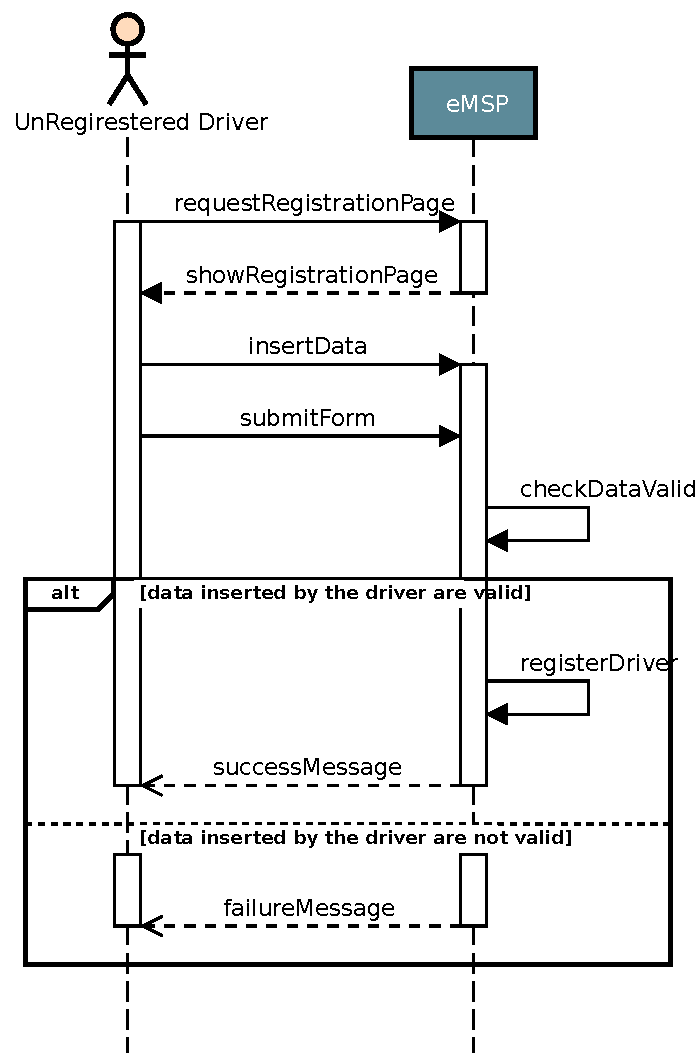
\includegraphics[
                width=\textwidth,
                height=0.35\textheight,
                keepaspectratio]{SeqDia/Register}
            \caption{Registration of a driver}
            \label{fig:Register}
            \end{center}
        \end{figure}
        \item \textbf{Driver Login}
        \begin{figure}[H]
            \begin{center}
            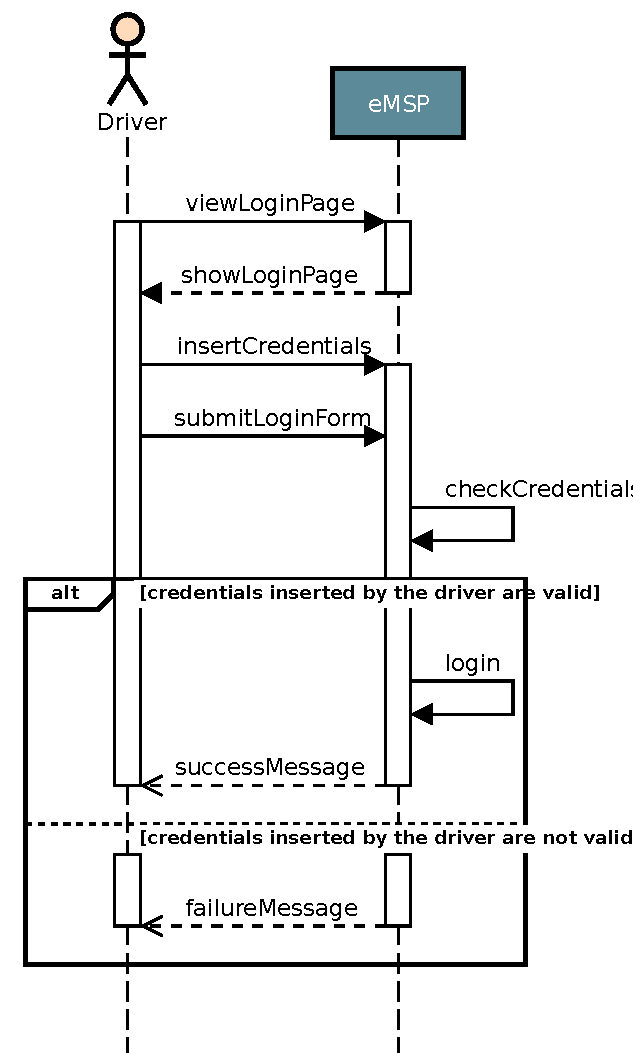
\includegraphics[
                width=\textwidth,
                height=0.35\textheight,
                keepaspectratio]{SeqDia/DriverLogin}
            \caption{Login of a Driver}
            \label{fig:DriverLogin}
            \end{center}
        \end{figure}
        \newpage
        \item \textbf{Check Map}
        \begin{figure}[H]
            \begin{center}
            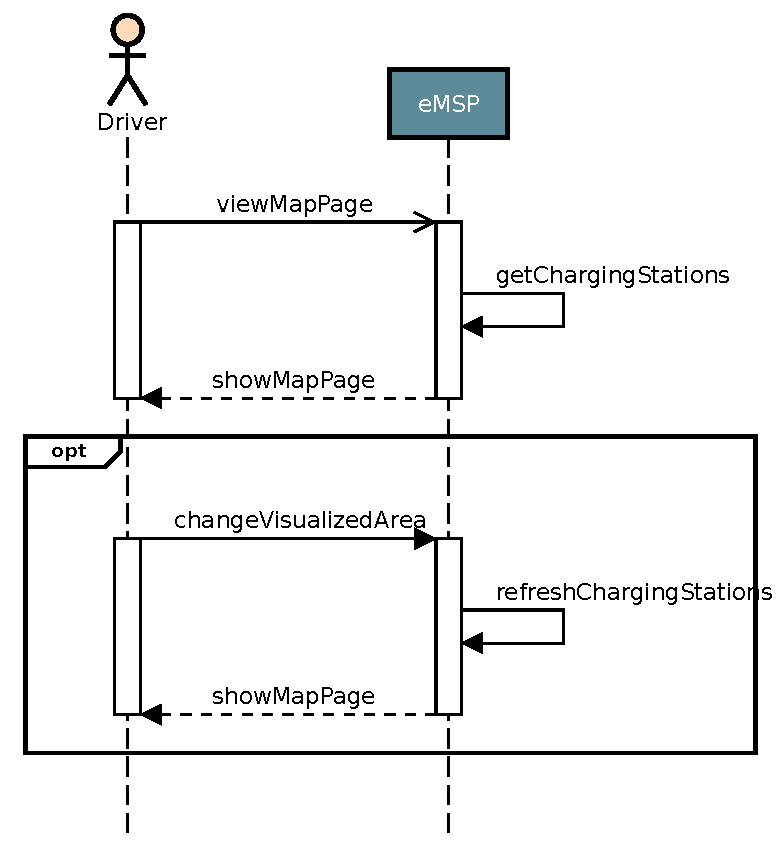
\includegraphics[
                width=\textwidth,
                height=0.43\textheight,
                keepaspectratio]{SeqDia/Map}
            \caption{Check Map of the eMSP}
            \label{fig:Map}
            \end{center}
        \end{figure}
        \item \textbf{Check Station Info}
        \begin{figure}[H]
            \begin{center}
            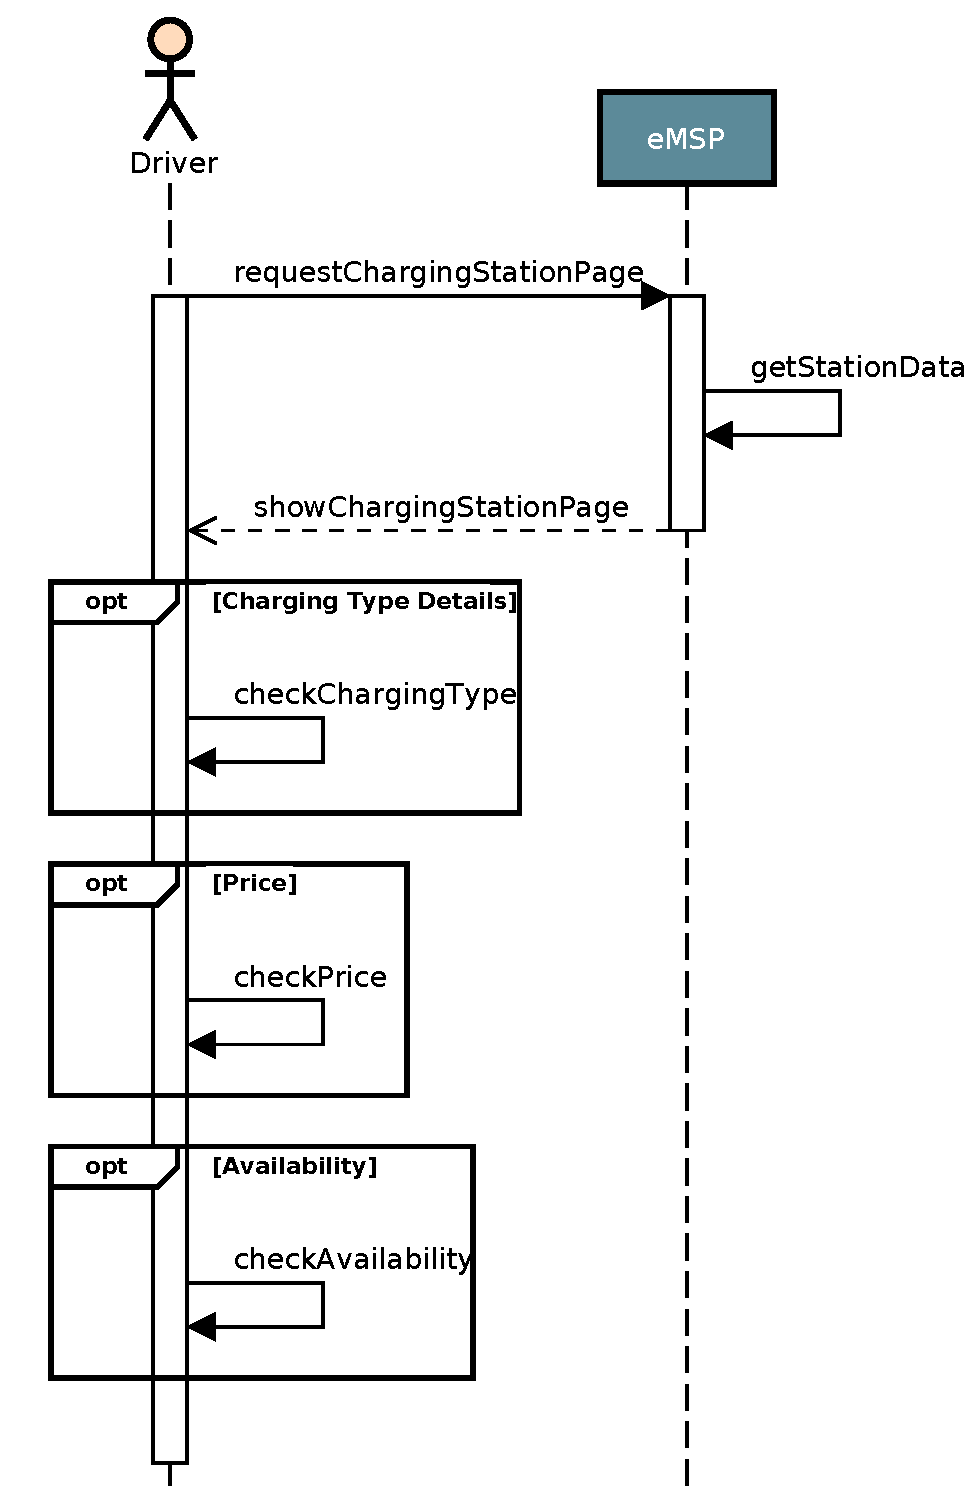
\includegraphics[
                width=\textwidth,
                height=0.4\textheight,
                keepaspectratio]{SeqDia/CheckStationInfo}
            \caption{Check Station Info}
            \label{fig:CheckStationInfo}
            \end{center}
        \end{figure}
        \newpage
        \item \textbf{Booking}
        \begin{figure}[H]
            \begin{center}
            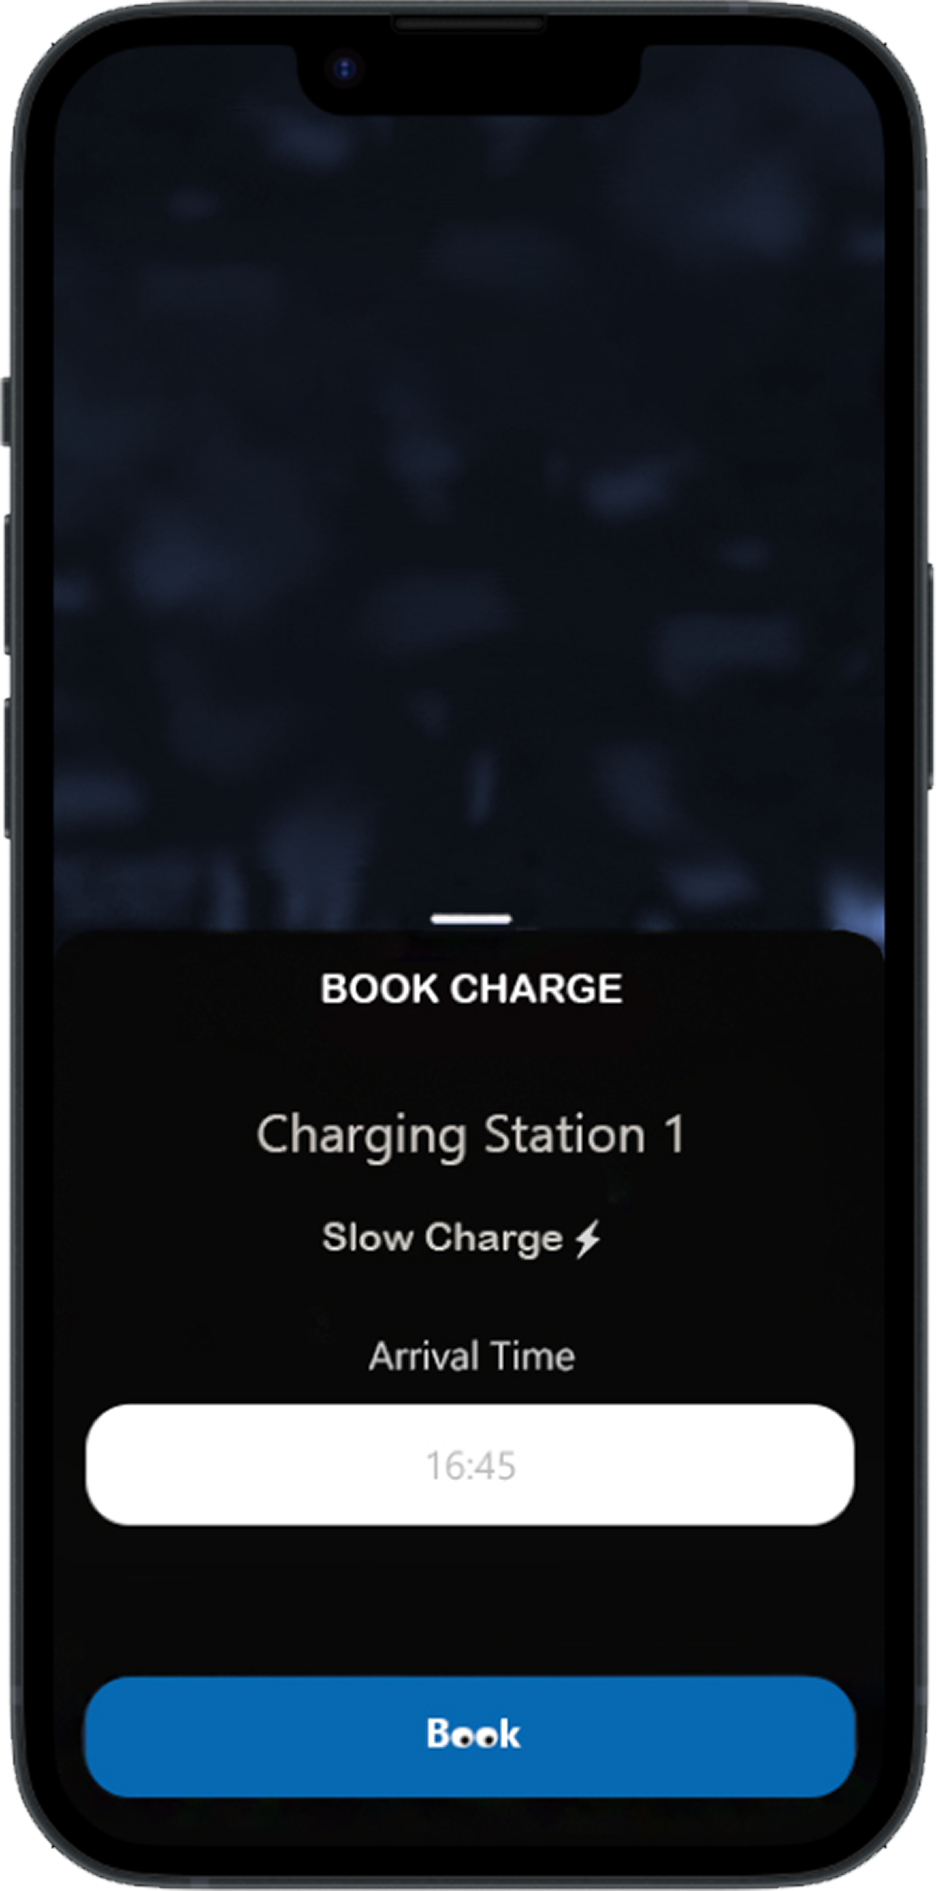
\includegraphics[
                width=\textwidth,
                height=\textheight,
                keepaspectratio]{SeqDia/BookCharge}
            \caption{Book a charging process}
            \label{fig:BookCharge}
            \end{center}
        \end{figure}
        \newpage
        \item \textbf{Delete Booking}
        \begin{figure}[H]
            \begin{center}
            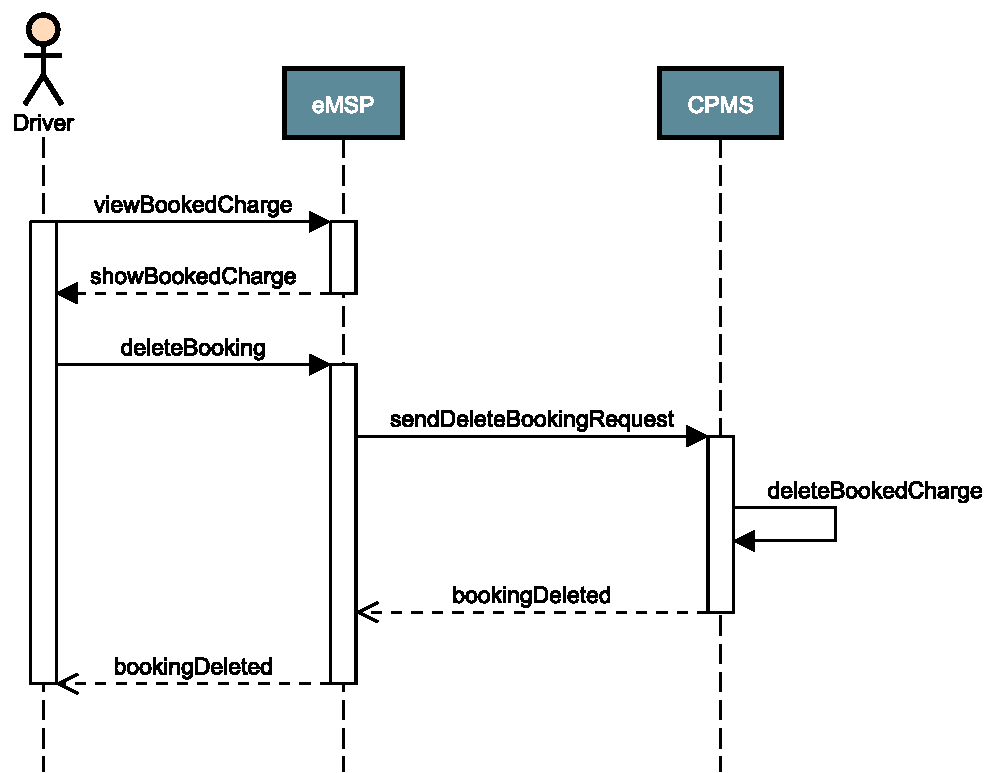
\includegraphics[
                width=\textwidth,
                height=0.6\textheight,
                keepaspectratio]{SeqDia/DeleteBooking}
            \caption{Delete a booked charging process}
            \label{fig:DeleteBooking}
            \end{center}
        \end{figure}
        \item \textbf{Suggestion Notification}
        \begin{figure}[H]
            \begin{center}
            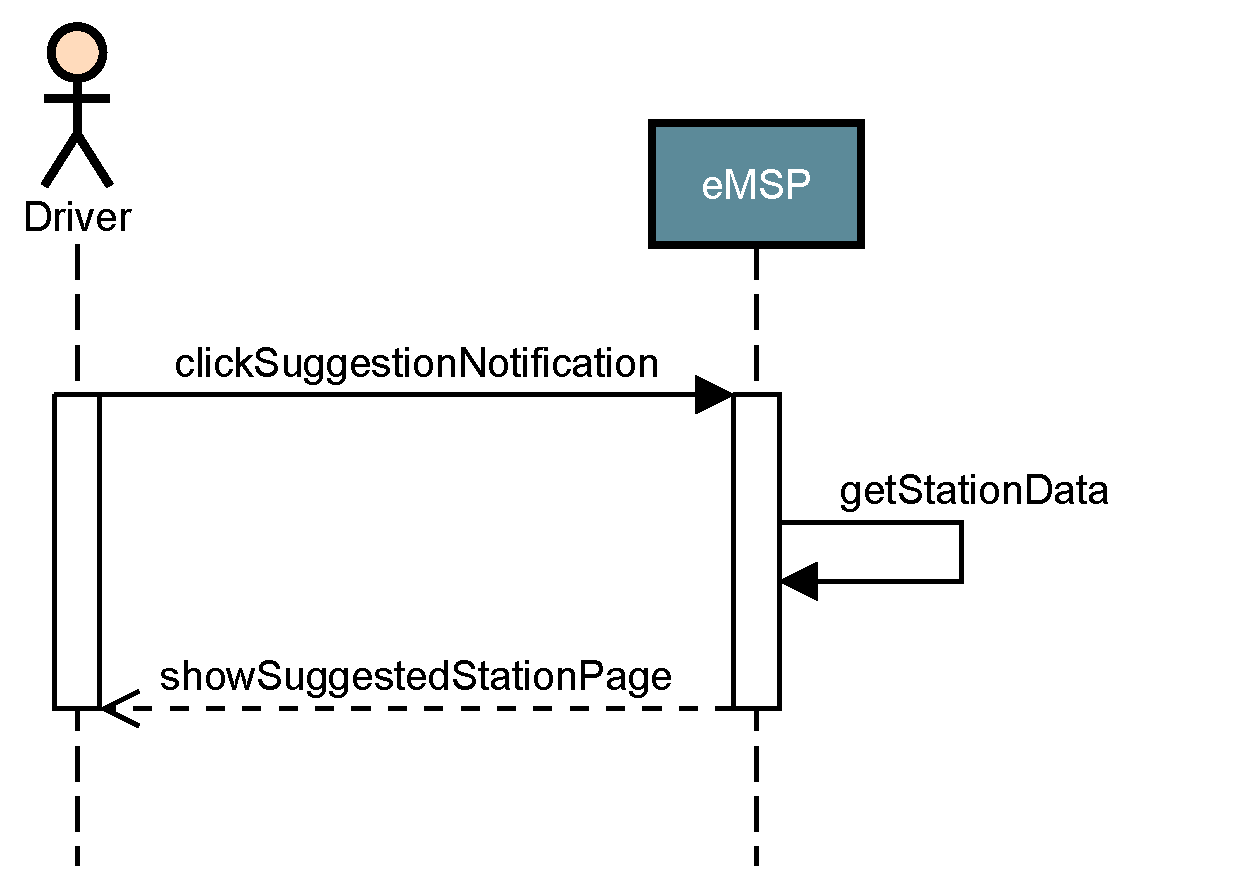
\includegraphics[
                width=\textwidth,
                height=0.3\textheight,
                keepaspectratio]{SeqDia/AdviceNotification}
            \caption{Driver receives and opens a suggestion}
            \label{fig:AdviceNotification}
            \end{center}
        \end{figure}
        \newpage
        \item \textbf{Charging Process}
        \begin{figure}[H]
            \begin{center}
            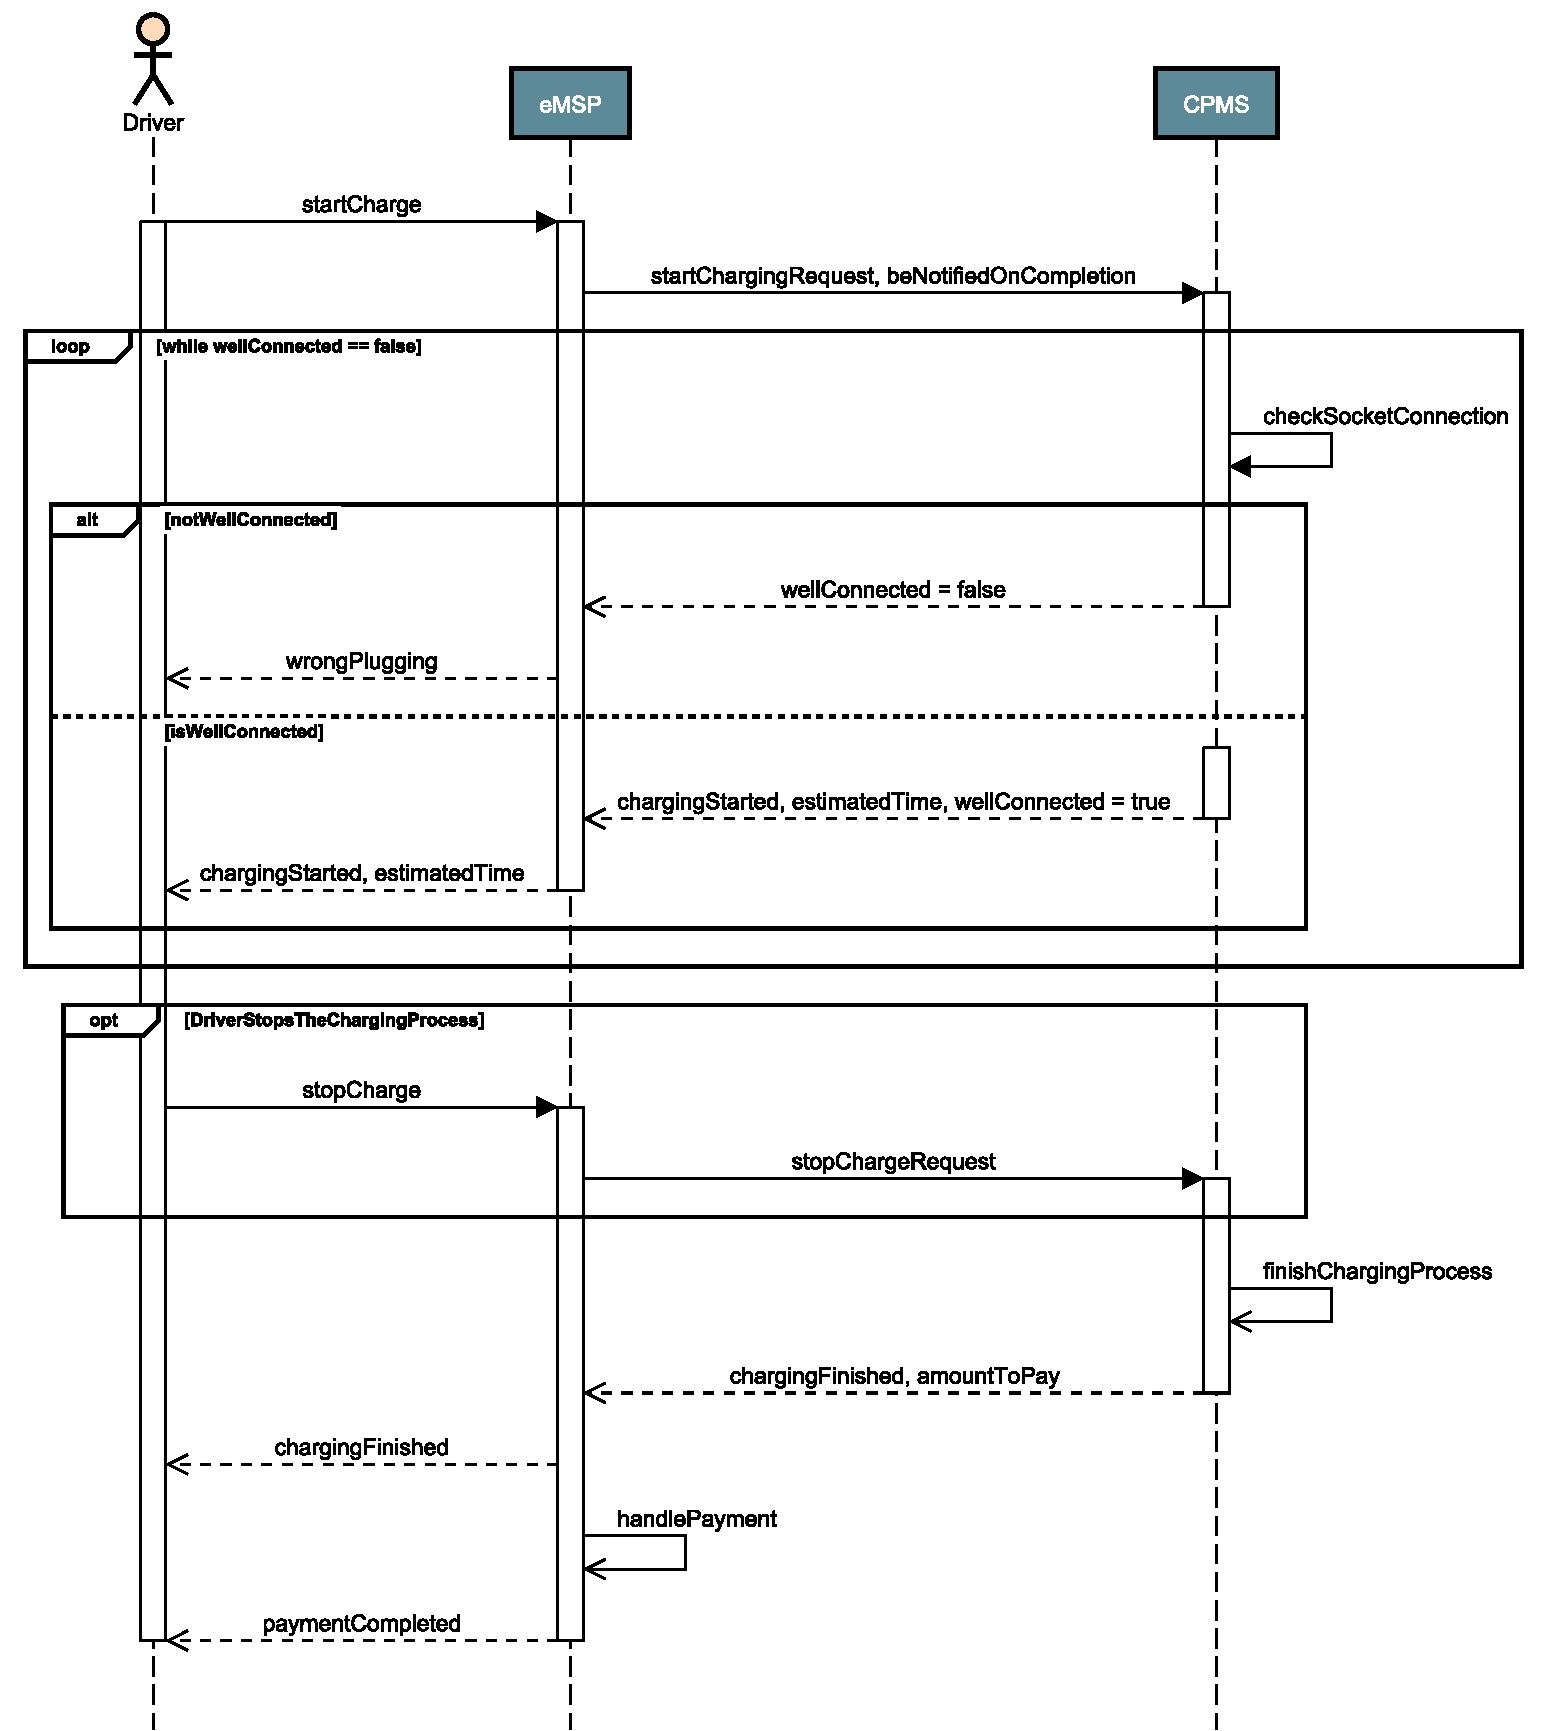
\includegraphics[
                width=\textwidth,
                height=\textheight,
                keepaspectratio]{SeqDia/StartCharge}
            \caption{Process of a charging process}
            \label{fig:StartCharge}
            \end{center}
        \end{figure}
        \newpage
        \item \textbf{CPO Login}
        \begin{figure}[H]
            \begin{center}
            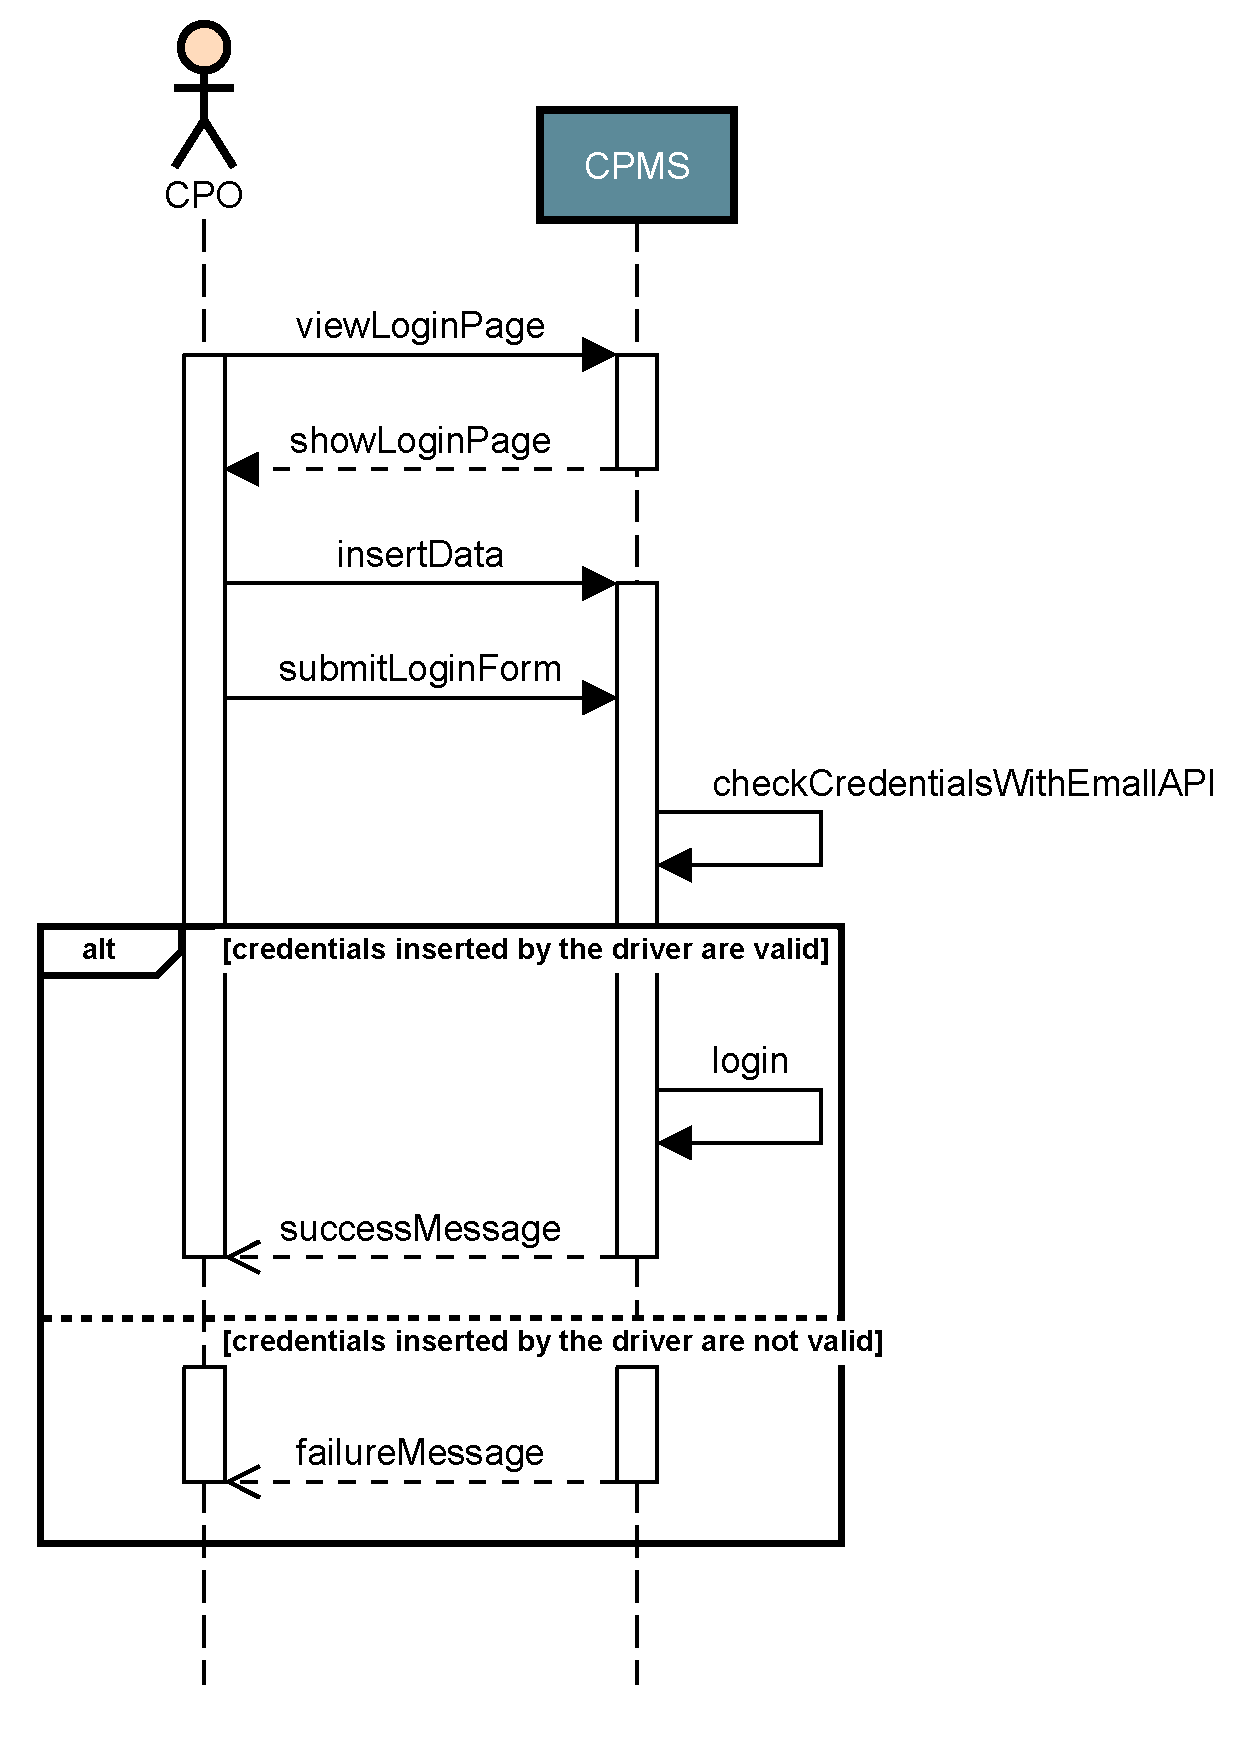
\includegraphics[
                width=\textwidth,
                height=0.45\textheight,
                keepaspectratio]{SeqDia/CPOLogin}
            \caption{Process of a charging process}
            \label{fig:CPOLogin}
            \end{center}
        \end{figure}
        \item \textbf{View Managed Station Status}
        \begin{figure}[H]
            \begin{center}
            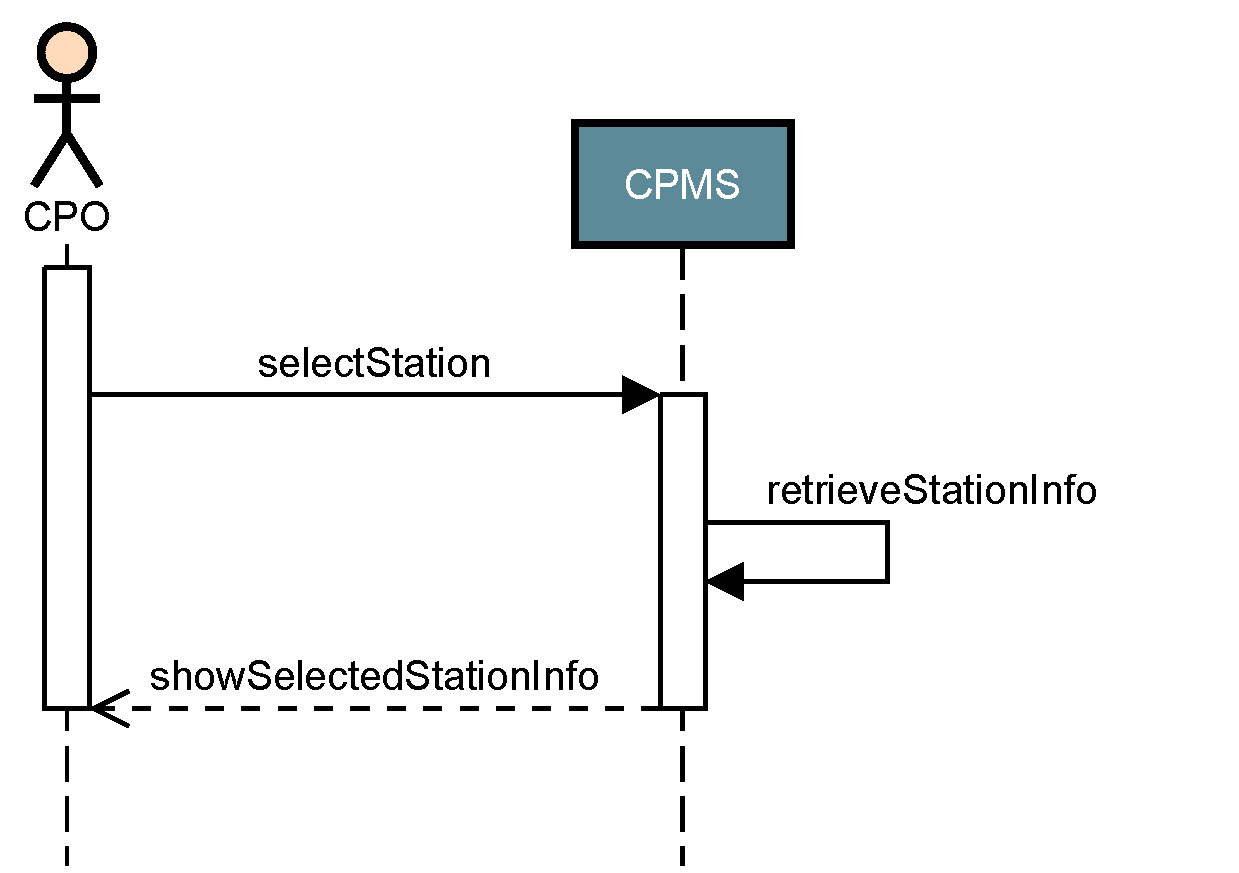
\includegraphics[
                width=\textwidth,
                height=0.35\textheight,
                keepaspectratio]{SeqDia/ManageStation}
            \caption{CPO views a managed station}
            \label{fig:ManageStation}
            \end{center}
        \end{figure}
        \newpage
        \item \textbf{Add Station To CPMS}
        \begin{figure}[H]
            \begin{center}
            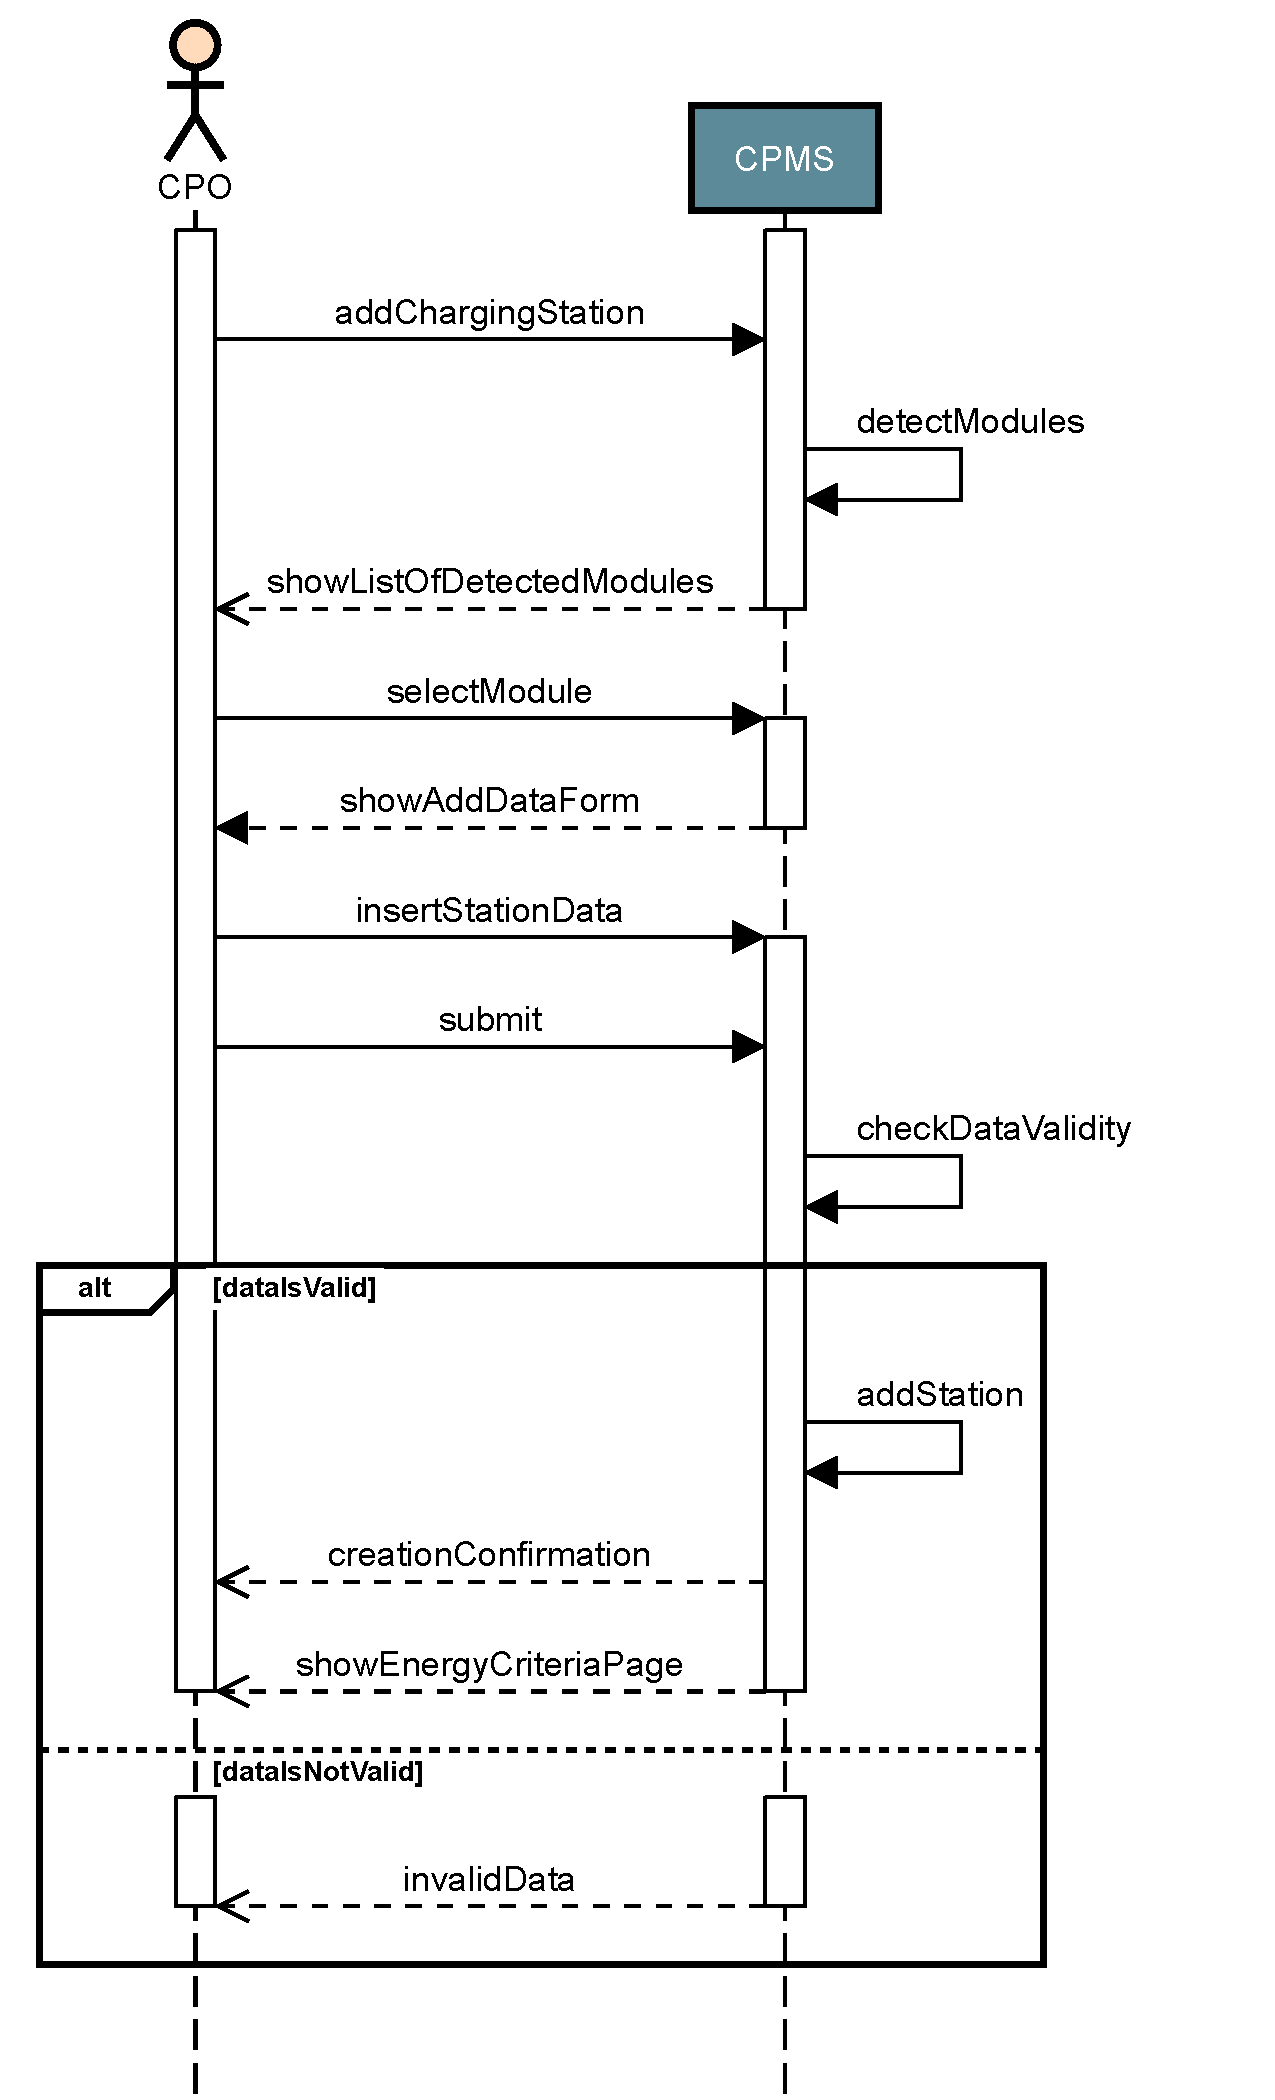
\includegraphics[
                width=\textwidth,
                height=0.85\textheight,
                keepaspectratio]{SeqDia/AddStation}
            \caption{CPO adds a station}
            \label{fig:AddStation}
            \end{center}
        \end{figure}
        \newpage
        \item \textbf{Set Offer}
        \begin{figure}[H]
            \begin{center}
            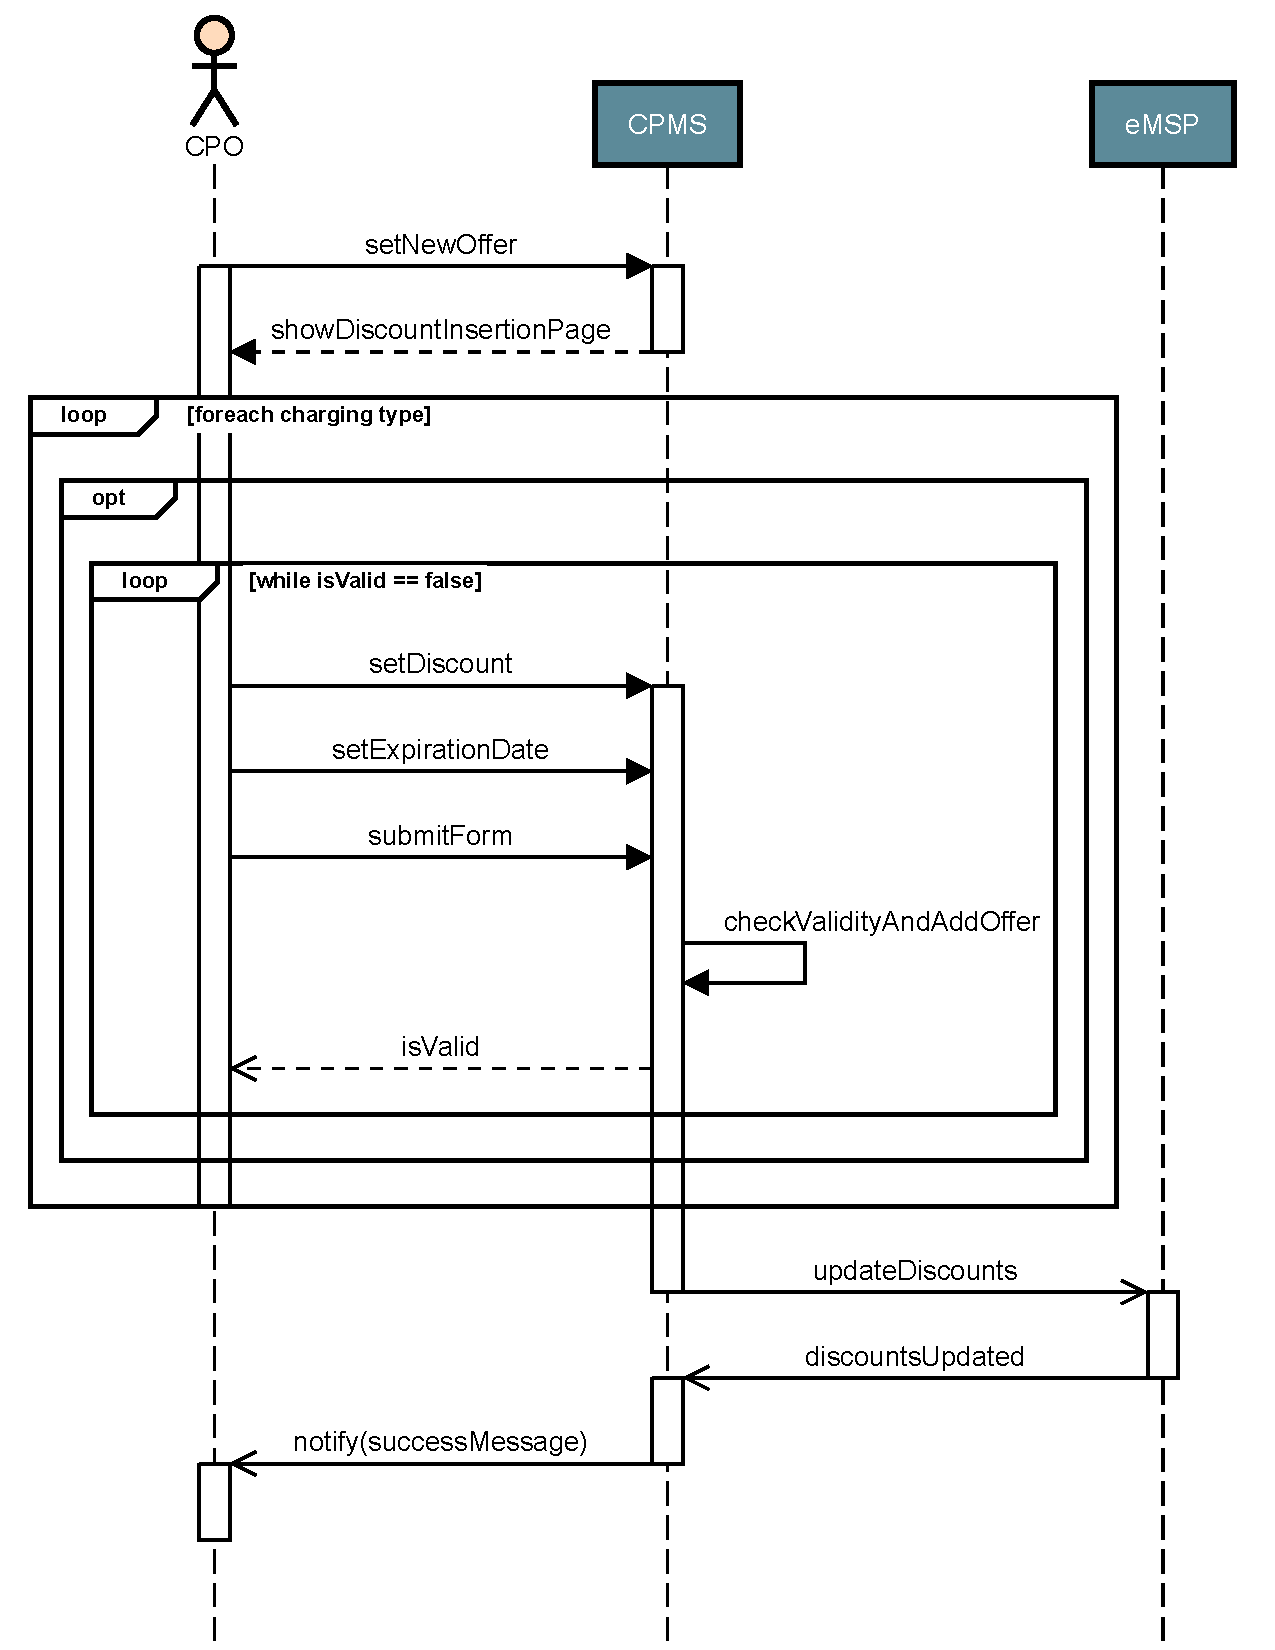
\includegraphics[
                width=\textwidth,
                height=\textheight,
                keepaspectratio]{SeqDia/SetOffer}
            \caption{CPO sets a new offer}
            \label{fig:SetOffer}
            \end{center}
        \end{figure}
        \newpage
        \item \textbf{Update Energy Criteria}
        \begin{figure}[H]
            \begin{center}
            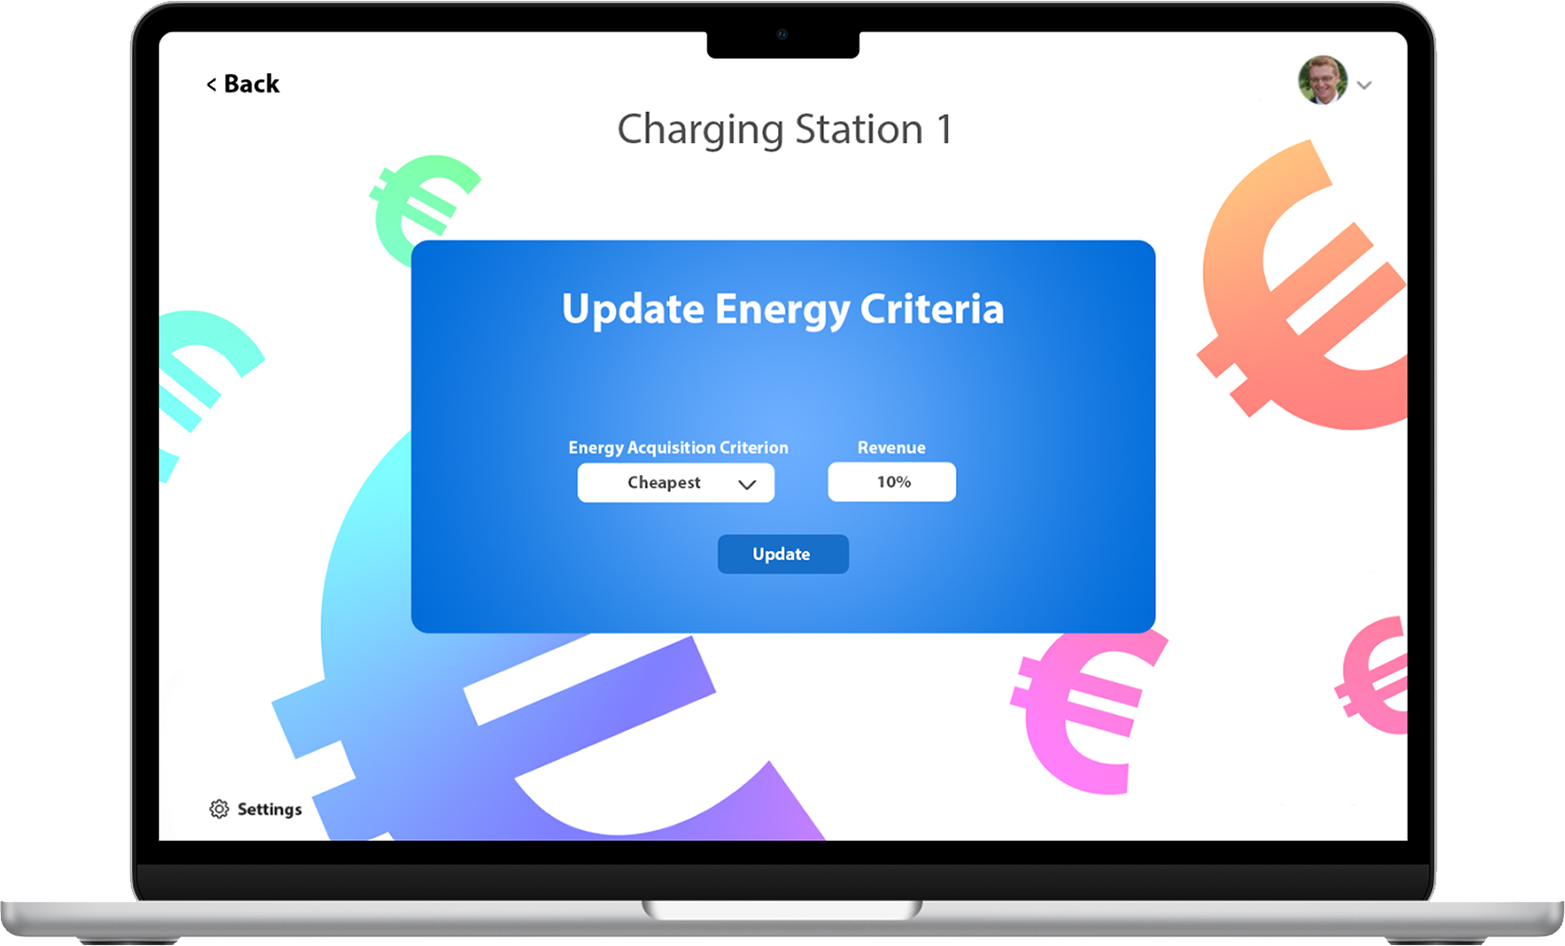
\includegraphics[
                width=\textwidth,
                height=0.85\textheight,
                keepaspectratio]{SeqDia/UpdateCriteria}
            \caption{CPO updates energy criteria}
            \label{fig:UpdateCriteria}
            \end{center}
        \end{figure}
        \newpage
        \item \textbf{eMSP Association}
        \begin{tabbing}
            \textbf{Note}: \= In \textit{sendCPOData} is also passed a payment method where the associated eMSP\\
            \> will send future drivers' payments.
        \end{tabbing}
        \begin{figure}[H]
            \begin{center}
            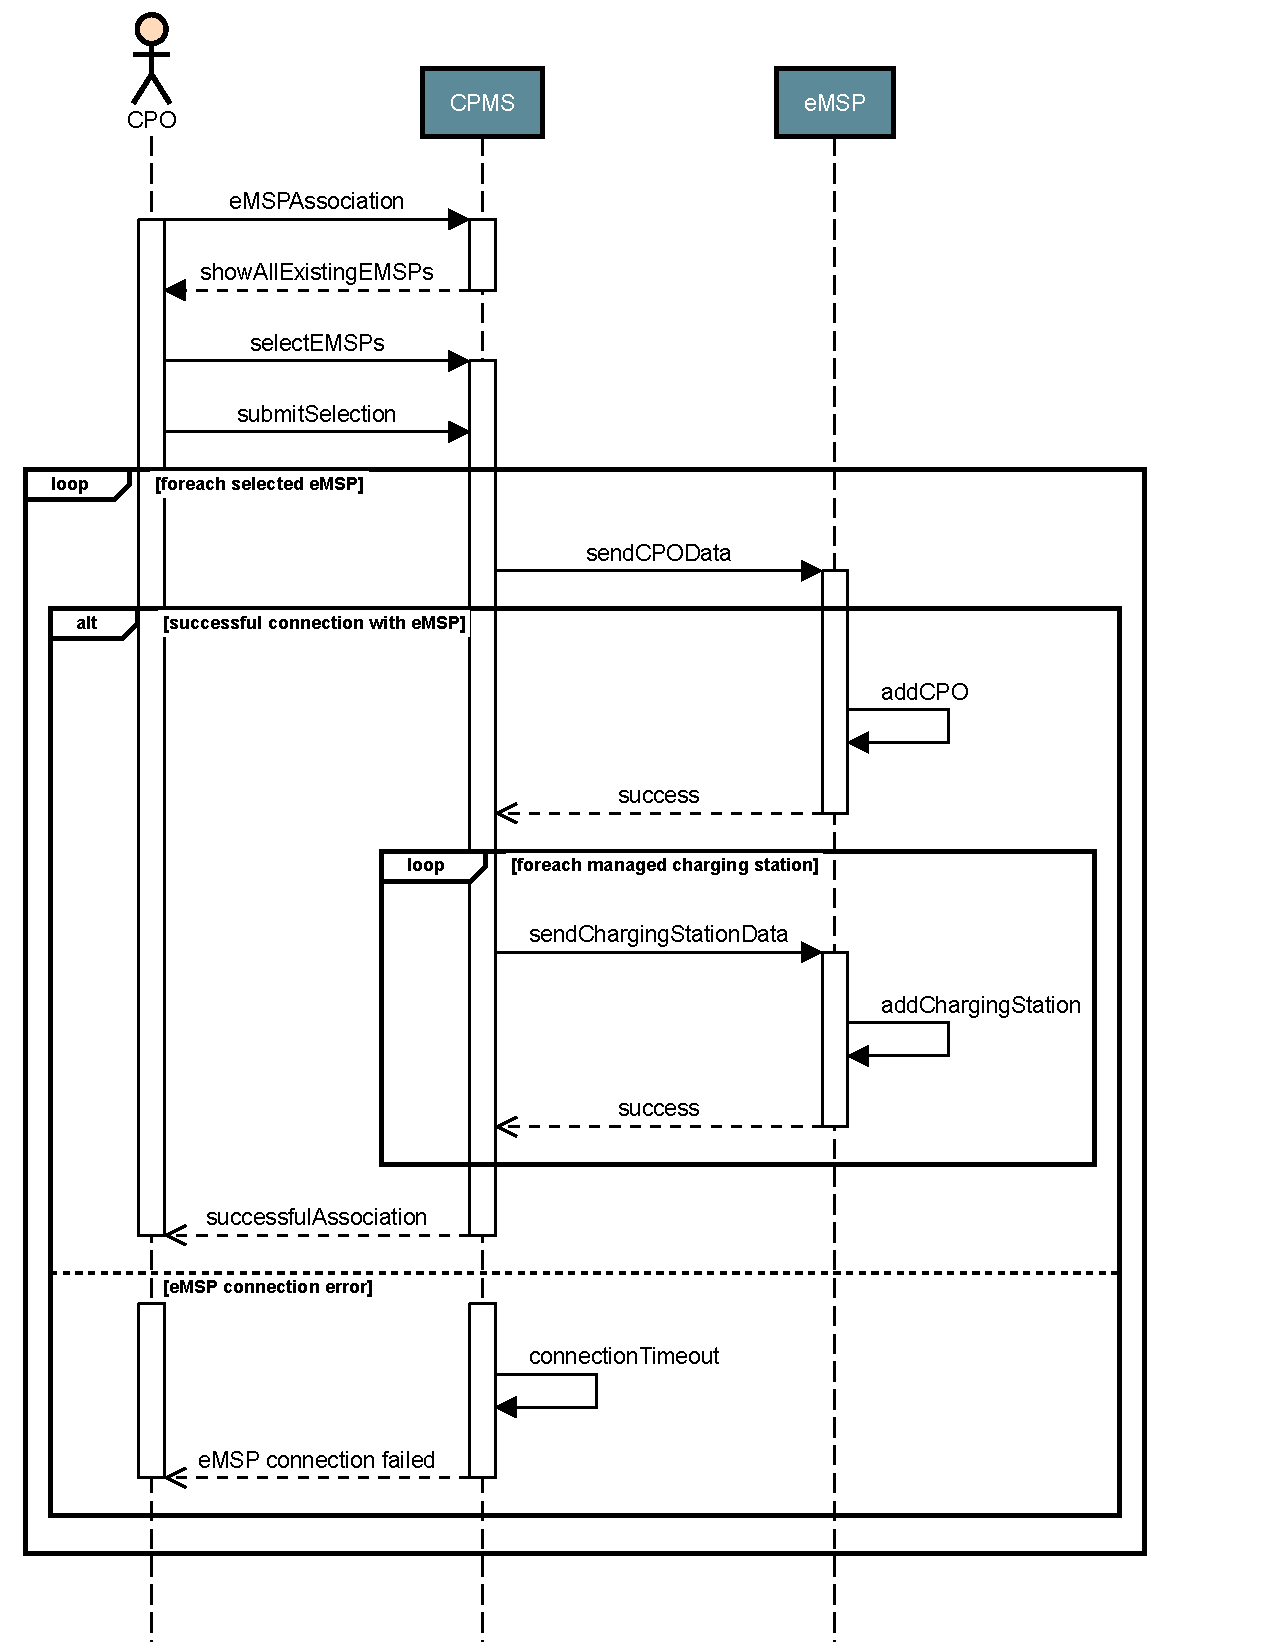
\includegraphics[   
                width=\textwidth,
                height=0.85\textheight,
                keepaspectratio]{SeqDia/eMSPAssociation}
            \caption{CPO associates a new eMSP}
            \label{fig:eMSPAssociation}
            \end{center}
        \end{figure}
\end{enumerate}
\restoregeometry
\subsection{eMSP Requirements}
In this section, the requirements for the two subsystems will be described as also their interactions. For both the Drivers and the CPOs it is required to be logged in to the system in order to perform any action different from Login and Registration
\begin{longtable}
{| p{0.12\linewidth} |p{0.28\linewidth} | p{0.6\linewidth} |}
    \hline
    \rowcolor{bluepoli!40}
     \textbf{ID} & \textbf{Name}& \textbf{Description} \T\B \\
    \hline 
    \hline
    \textbf{FRE\row} & Driver Registration & An Unregistered Driver shall be able to register himself on the eMSP application.\T\B\\
    \hline
    \textbf{FRE\row} & Driver Login &The Driver shall be able to login to the eMSP with his credentials.\T\B\\
    \hline
    \textbf{FRE\row} & Internet Connection & The system shall notify the Driver if there is no internet connection.\T\B\\
    \hline
    \textbf{FRE\row} & View Charging Stations & The Driver shall be able to see the location of all the charging stations in a certain geographic area.\T\B\\
    \hline
    \textbf{FRE\row} & Charging Type Selection & The Driver shall be able to select the charging types he is interested in while searching for a charging station in order to filter them.\T\B\\
    \hline
    \textbf{FRE\row} & Charging Cost & The Driver shall be able to check the cost per kWh for the specified charging types in a specific charging station.\T\B\\
    \hline
    \textbf{FRE\row} & Charging Station Availability & The Driver shall be able to see which charging stations are currently available for the specified charging types.\T\B\\
    \hline
    \textbf{FRE\row} & Future Availability & The Driver shall be able to see an estimated time in which a specific charging station will become available.\T\B\\
    \hline
    \textbf{FRE\row} & Charge Booking & The Driver shall be able to book a charging socket in an available charging station, from 0 up to a max specified amount of time before.\T\B\\
    \hline
    \textbf{FRE\row} & Booked Charging Socket ID & The system shall show the Driver the booked socket ID number.\T\B\\
    \hline
    \textbf{FRE\row} & Delete Booking & The Driver shall be able to delete a booked charging process before its starting time.\T\B\\
    \hline
    \textbf{FRE\row} & Confirm Booking & The Driver shall receive a notification that confirms the booking went well.\T\B\\
    \hline
    \textbf{FRE\row} & Start Charging Process & As soon as the booked time starts the Driver shall be able to start the recharging process.\T\B\\
    \hline
    \textbf{FRE\row} & Stop Charging Process & During the recharging process the Driver shall be able to stop it in advance.\T\B\\
    \hline
    \textbf{FRE\row} & Time remaining  & The Driver shall be able to check the estimated remaining time until the end of the charging process.\T\B\\
    \hline
    \textbf{FRE\row} & Charge Finished  & The system shall notify the Driver when the charging process is complete.\T\B\\
    \hline
    \textbf{FRE\row} & Payment & At the end of the charging process, the system shall handle the payment between the Driver and the CPO through an external API.\T\B\\%, retrieving from the Driver’s given payment method the amount of money to pay requested by the CPMS for that charge.\T\B\\
    \hline   
    \textbf{FRE\row} & Generic Error Notification & Every time the system fails to elaborate an operation related to a Driver, then he shall receive a notification containing the error details.\T\B\\
    \hline
    \textbf{FRE\row} & Successful Payment Notification & The system shall notify the Driver when a successful payment occurs.\T\B\\
    \hline    
    \textbf{FRE\row} & Check Vehicle Connection & The system shall be able to check if there exists a connection between the Driver's vehicle and the system itself.\T\B\\
    \hline
    \textbf{FRE\row} & Vehicle’s Remaining Charge & If the vehicle is connected, the system shall be able to retrieve the battery level of the Driver's vehicle.\T\B\\
    \hline
    \textbf{FRE\row} & Vehicle’s Location & If the vehicle is connected, the system shall be able to retrieve the Driver's vehicle location.\T\B\\
    \hline
    \textbf{FRE\row} & Data Integration & The Driver shall be able to authorize the system to access his personal data such as his calendar, navigation system and location.\T\B\\
    \hline
    \textbf{FRE\row} & Calendar Data & The system shall be able to retrieve data from the Driver's personal calendar.\T\B\\
    \hline
    \textbf{FRE\row} & Navigation System & The system shall retrieve information about the Driver’s navigation system.\T\B\\
    \hline
    \textbf{FRE\row} & Charging Suggestion Creation & If the vehicle is connected to the Driver's device, the eMSP shall create charging suggestion notifications based on the status of the vehicle's battery, the Driver's schedule (his calendar and navigation system), special offers made available at some charging stations and the availability of charging sockets at those identified charging stations.\T\B\\
    \hline
    \textbf{FRE\row} & Suggestion Notification & The system shall advise the Driver with a notification when and where he should recharge his vehicle’s battery.\T\B\\
    \hline    
    \textbf{FRE\row} & Suggestion Interaction & The Driver shall be able to click on the charging suggestion notification sent by the eMSP and that shall redirect to the suggested charging station's info page.\T\B\\
    \hline
    %\textbf{FRE\row} & CPMS communication & The system shall be able to communicate with the specific CPMS while performing an operation within one of its managed stations. \T\B\\
    %\hline
    \caption{Table of eMSP Requirements}
\end{longtable}
\subsection{CPMS Requirements}
\begin{longtable}{| p{0.12\linewidth} |p{0.28\linewidth} | p{0.6\linewidth} |}
    \hline
    \rowcolor{bluepoli!40}
     \textbf{ID} & \textbf{Name}& \textbf{Description} \T\B \\
    \hline 
    \hline
    \textbf{FRE\row} & CPO Login & The CPO shall be able to login to the CPMS with his credentials.\T\B\\
    \hline
    \textbf{FRE\row} & Internet Connection & The system shall notify the CPO if there is no internet connection.\T\B\\
    \hline
    \textbf{FRE\row} & View Charging Stations & The CPO shall be able to see the list of only all his owned charging stations.\T\B\\
    \hline
    \textbf{FRE\row} & Add Charging Station & The CPO shall be able to add a new charging station.\T\B\\
    \hline
    \textbf{FRE\row} & Batteries Energy & The CPO shall be able to check the remaining energy stored in the batteries in one of his own charging stations.\T\B\\
    \hline
    \textbf{FRE\row} & Number Of Vehicles  & The CPO shall be able to check the number of vehicles being charged in one of his charging stations.\T\B\\
    \hline
    \textbf{FRE\row} & Power Absorption  & The CPO shall be able to check the amount of power absorbed from each vehicle being charged in one of his charging stations.\T\B\\
    \hline
    \textbf{FRE\row} & Charging Time Left  & The system shall be able to give an estimation about how much time is needed to end the charging process for a particular vehicle being charged in a charging station.\T\B\\
    \hline
    \textbf{FRE\row} & Energy Price Information & The system shall be able to retrieve the current energy price and the capacity for each of the available DSOs.\T\B\\
    \hline   
    \textbf{FRE\row} & Battery Energy Provider & The system shall be able to use the batteries as energy providers with prices equal to the cost that was used to recharge them. \T\B\\
    \hline
    \textbf{FRE\row} & Energy Acquisition Criteria & The CPO shall be able to select the criteria that will be used by the CPMS in order to acquire energy, such as Energy provider with the lowest price, Energy Provider with biggest energy capacity.\T\B\\
    \hline
    \textbf{FRE\row} & Energy Revenue Criteria  & The CPO shall be able to select the revenue percentage amount from the energy sale of each charging station.\T\B\\
    \hline
    \textbf{FRE\row} & Energy Acquisition Decision & The system shall be able, for each charging station, to automatically decide from which energy provider to retrieve the energy, based on the criteria chosen by the CPO.\T\B\\
    \hline
    \textbf{FRE\row} & Energy Sale Price  & The system shall be able, for each charging station, to automatically calculate the selling price of the energy based on the revenue criteria and on the price of the energy provider.\T\B\\
    \hline 
    \textbf{FRE\row} & Payment Calculation & The system shall be able to calculate when a charging process ends, the amount requested to pay based on the energy consumed and its selling price.\T\B\\
    \hline 
    \textbf{FRE\row} & Internal Battery Management & The system shall be able to automatically decide whether to store or not energy in the internal batteries, if available, of one of the managed charging stations.\T\B\\
    \hline
    \textbf{FRE\row} & Special Offers  & The system shall allow the CPO to apply discounts for the energy prices of a managed charging station until a set expiration date.\T\B\\
    \hline
    \textbf{FRE\row} & eMSP list & The CPO shall be able to see a list of all the existing eMSPs.\T\B\\
    \hline
    \textbf{FRE\row}& eMSP association & The CPO shall be able to decide which eMSP he wants to associate with his CPMS in order to permit communication between the two systems. \T\B\\
    \hline
    \caption{Table of CPMS Requirements}
\end{longtable}
\subsection{Interaction Requirement}
Here there is the description of the requirements that are in common between the two subsystems. To avoid having a large number of requirements, the following ones should be read in this way:\\
\begin{itemize}
    \item\textbf{Format 1}: The eMSP shall (be able to) "perform an operation" on a single CPMS:
    \begin{itemize}
        \item The eMSP shall communicate with the CMPS requesting to "perform an operation".
        \item The CPMS shall return to eMSP the result of the "performed operation".
    \end{itemize}
    \item \textbf{Format 2}: CPMS updates "data":
    \begin{itemize}
        \item The CPMS shall detect when some "data" are updated.
        \item The CPMS shall send to every associated eMSP the new updated "data".
        \item The eMSP shall store the "data" received by the CMPS and show it to the driver when he requests it.
    \end{itemize}
\end{itemize}
\begin{longtable}{| p{0.12\linewidth} |p{0.28\linewidth} | p{0.6\linewidth} |}
    \hline
    \rowcolor{bluepoli!40}
     \textbf{ID} & \textbf{Name}& \textbf{Description} \T\B \\
    \hline 
    \hline
    \textbf{FRE\row} & Book a charge & The eMSP shall be able to book a charge and receive the booked charging socket on a single CPMS.\T\B\\
    \hline
    \textbf{FRE\row} & Delete a booked charge & The eMSP shall be able to delete a previously booked charge on a single CPMS.\T\B\\
    \hline
    \textbf{FRE\row} & Start charge & The eMSP shall be able to start a charge on a single CPMS.\T\B\\
    \hline
    \textbf{FRE\row} & Wrong plugging & The eMSP shall be notified when the vehicle is not well connected to the charging socket on a single CPMS.\T\B\\
    \hline 
    \textbf{FRE\row} & Stop charge & The eMSP shall be able to stop a charge on a single CPMS.\T\B\\
    \hline
    \textbf{FRE\row} & Amount to pay & The eMSP shall be notified with the required amount of money to pay when the charging process ends on a single CPMS .\T\B\\
    \hline
    \textbf{FRE\row} & Remaining Charge Time & The eMSP shall be able to ask for the estimated ending time for a specific charging process.\T\B\\
    \hline
    \textbf{FRE\row}& Charging station availability & If CPMS can calculate the estimated time before each charging type becomes available, CPMS updates the availability of a charging station with the estimated time otherwise, CPMS updates only the availability. \T\B\\
    \hline
    \textbf{FRE\row}& Charging station price & CPMS updates the price of a charging type in a station.\T\B\\
    \hline
    \textbf{FRE\row} &Charging station offer & CPMS updates the offer of a charging type in a station.\T\B\\
    \hline
    \textbf{FRE\row} & Charging station creation & CPMS updates about the data of the newly created charging station such as location, prices, supported charging types.\T\B\\
    \hline
    \caption{Table of Interaction Requirements}
    \setcounter{row}{0}
\end{longtable}
\newpage
\subsection{Requirements mapping on Goals}
\begin{longtable}{| p{0.1\linewidth} | P{0.05\linewidth} |P{0.05\linewidth} |P{0.05\linewidth} |P{0.05\linewidth} |P{0.05\linewidth} |P{0.05\linewidth} | P{0.05\linewidth}|}
    \hline
    \rowcolor{bluepoli!40}
     \textbf{R/G} & \textbf{G1} & \textbf{G2}& \textbf{G3}& \textbf{G4}& \textbf{G5}& \textbf{G6} &\textbf{G7}\T\B \\
    \hline 
    \hline
    \textbf{FRE\row} &X &X &X &X & & &\T\B\\
    \hline
    \textbf{FRE\row} &X &X &X &X & & &\T\B\\
    \hline
    \textbf{FRE\row} &X &X &X &X & & &\T\B\\
    \hline
    \textbf{FRE\row} &X &X & & & & &\T\B\\
    \hline
    \textbf{FRE\row} &X &X & & & & &\T\B\\
    \hline
    \textbf{FRE\row} &X & & & & & &\T\B\\
    \hline
    \textbf{FRE\row} &X &X & & & & &\T\B\\
    \hline
    \textbf{FRE\row} &X &X & & & & &\T\B\\
    \hline
    \textbf{FRE\row} & &X & & & & &\T\B\\
    \hline
    \textbf{FRE\row} & &X &X & & & & \T\B\\
    \hline
    \textbf{FRE\row} & &X & & & & &\T\B\\
    \hline
    \textbf{FRE\row} & &X & & & & &\T\B\\
    \hline
    \textbf{FRE\row} & & &X & & & &\T\B\\
    \hline
    \textbf{FRE\row} & & &X & & & &\T\B\\
    \hline
    \textbf{FRE\row} & & &X & & & &\T\B\\
    \hline
    \textbf{FRE\row} & & &X & & & &\T\B\\
    \hline
    \textbf{FRE\row} & & & &X & & & \T\B\\
    \hline
    \textbf{FRE\row} &X &X &X &X &X & & \T\B\\
    \hline
    \textbf{FRE\row} & & & &X & & & \T\B\\
    \hline
    \textbf{FRE\row} & & & & &X & & \T\B\\
    \hline
    \textbf{FRE\row} & & & & &X & & \T\B\\
    \hline
    \textbf{FRE\row} &X & & & &X & & \T\B\\
    \hline
    \textbf{FRE\row} & & & & &X & & \T\B\\
    \hline
    \textbf{FRE\row} & & & & &X & & \T\B\\
    \hline
    \textbf{FRE\row} & & & & &X & & \T\B\\
    \hline
    \textbf{FRE\row} & & & & &X & & \T\B\\
    \hline
    \textbf{FRE\row} & & & & &X & & \T\B\\
    \hline
    \textbf{FRE\row} & & & & &X & & \T\B\\
    \hline
    \hhline{========}
    \textbf{FRE\row} & & & & & &X &X\T\B\\
    \hline
    \textbf{FRE\row} & & & & & &X &X\T\B\\
    \hline
    \textbf{FRE\row} & & & & & &X &X\T\B\\
    \hline
    \textbf{FRE\row} & & & & & &X &X\T\B\\
    \hline
    \textbf{FRE\row} & & & & & & &X\T\B\\
    \hline
    \textbf{FRE\row} & & & & & & &X\T\B\\
    \hline
    \textbf{FRE\row} & & & & & & &X\T\B\\
    \hline
    \textbf{FRE\row} & & &X & & & &X\T\B\\
    \hline
    \textbf{FRE\row} & & & & & &X &\T\B\\
    \hline
    \textbf{FRE\row} & & & & & &X &\T\B\\
    \hline
    \textbf{FRE\row} & & & & & &X &\T\B\\
    \hline
    \textbf{FRE\row} & & & &X& &X &\T\B\\
    \hline
    \textbf{FRE\row} & & & & & &X &\T\B\\
    \hline
    \textbf{FRE\row} & & & &X& &X &\T\B\\
    \hline
    \textbf{FRE\row} & & & &X & & &\T\B\\
    \hline
    \textbf{FRE\row} & & & & & &X &\T\B\\
    \hline
    \textbf{FRE\row} &X & & & &X &X &\T\B\\
    \hline
    \textbf{FRE\row} &X &X &X &X &X & &\T\B\\
    \hline
    \textbf{FRE\row} &X &X &X &X &X& &\T\B\\
    \hhline{========}
    \textbf{FRE\row} & &X & & & & &\T\B\\
    \hline
    \textbf{FRE\row} & &X & & & & &\T\B\\
    \hline
    \textbf{FRE\row} & & &X & & & &X\T\B\\
    \hline
    \textbf{FRE\row} & & &X & & & &\T\B\\
    \hline
    \textbf{FRE\row} & & &X & & & &X\T\B\\
    \hline
    \textbf{FRE\row} & & &X &X & & &\T\B\\
    \hline
    \textbf{FRE\row} & & &X & & & &X\T\B\\
    \hline
    \textbf{FRE\row} &X &X & & &X & &\T\B\\
    \hline
    \textbf{FRE\row} &X & & & &X & &\T\B\\
    \hline
    \textbf{FRE\row} &X & & & &X & &\T\B\\
    \hline
    \textbf{FRE\row} &X &X & & &X & &\T\B\\
    \hline
    \caption{Mapping of Requirements on Goals}
    \setcounter{row}{0}
\end{longtable}
\newpage
\subsection{Domain Assumption mapping on Goals}
\begin{longtable}{| p{0.1\linewidth} | P{0.05\linewidth} |P{0.05\linewidth} |P{0.05\linewidth} |P{0.05\linewidth} |P{0.05\linewidth} |P{0.05\linewidth} | P{0.05\linewidth}|}
    \hline
    \rowcolor{bluepoli!40}
     \textbf{R/G} & \textbf{G1} & \textbf{G2}& \textbf{G3}& \textbf{G4}& \textbf{G5}& \textbf{G6} &\textbf{G7}\T\B \\
    \hline 
    \hline
    \textbf{D\row} & & &X & & & &\T\B\\
    \hline
    \textbf{D\row} &X &X &X &X &X & &\T\B\\
    \hline
    \textbf{D\row} &X & &X & & & &\T\B\\
    \hline
    \textbf{D\row} & &X &X & & & &\T\B\\
    \hline
    \textbf{D\row} & X & X & X & & & &\T\B\\
    \hline
    \textbf{D\row} & & &X & & & &\T\B\\
    \hline
    \textbf{D\row} & & &X && & &\T\B\\
    \hline
    \textbf{D\row} & &X &X & & & &\T\B\\
    \hline
    \textbf{D\row} & & & & &X & &\T\B\\
    \hline
    \textbf{D\row} & & & & & X & & \T\B\\
    \hline
    \textbf{D\row} & & & & & & X &X\T\B\\
    \hline
    \textbf{D\row} & & & & & & X &\T\B\\
    \hline
    \textbf{D\row} & & & & X& &  &\T\B\\
    \hline
    \textbf{D\row} &X & & & & & &\T\B\\
    \hline
    \textbf{D\row} &X &X &X &X &X & &\T\B\\
    \hline
    \textbf{D\row} & & & & & &X &X\T\B\\
    \hline
\end{longtable}
\subsection{Explicit Goal Mapping}
% TEIBOL per l'explicit mapping
{\renewcommand{\arraystretch}{1.5}
\begin{longtable}{|p{0.20\linewidth}p{0.75\linewidth}|}
    \hline
    % Goal
    \rowcolor{bluepoli!40}\textbf{G1} & \textbf{Allow Drivers to check nearby charging stations and see info about their prices, special offers and availability.} \\
    \hline
    % Requirements
    \rowcolor{bluepoli!15} FRE1 & An Unregistered Driver shall be able to register himself on the eMSP application. \\
    \hline
    \rowcolor{bluepoli!15} FRE2 & The Driver shall be able to login to the eMSP with his credentials. \\
    \hline 
    \rowcolor{bluepoli!15} FRE3 & The system shall notify the Driver if there is no internet connection. \\
    \hline 
    \rowcolor{bluepoli!15} FRE4 & The Driver shall be able to see the location of all the charging stations in a certain geographic area. \\
    \hline 
    \rowcolor{bluepoli!15} FRE5 & The Driver shall be able to select the charging types he is interested in while searching for a charging station in order to filter them. \\
    \hline 
    \rowcolor{bluepoli!15} FRE6 & The Driver shall be able to check the cost per kWh for the specified charging types in a specific charging station. \\
    \hline  
    \rowcolor{bluepoli!15} FRE7 & The Driver shall be able to see which charging stations are currently available for the specified charging types. \\
    \hline  
    \rowcolor{bluepoli!15} FRE8 & The Driver shall be able to see an estimated time in which a specific charging station will become available. \\
    \hline  
    \rowcolor{bluepoli!15} FRE18 & Every time the system fails to elaborate an operation related to a Driver, then he shall receive a notification containing the error details. \\
    \hline  
    \rowcolor{bluepoli!15} FRE22 & If the vehicle is connected, the system shall be able to retrieve the Driver’s vehicle location \\
    \hline  
    \rowcolor{bluepoli!15}
    FRE45 &The system shall allow the CPO to apply discounts for the energy prices of a managed charging station until a set expiration date. \\
    \hline
    \rowcolor{bluepoli!15}
    FRE46 & The CPO shall be able to see a list of all the existing eMSPs. \\
    \hline
    \rowcolor{bluepoli!15} FRE47 & The CPO shall be able to decide which eMSP he wants to associate with his CPMS in order to permit communication between the two systems \\
    \hline
    \rowcolor{bluepoli!15} FRE55 & If CPMS can calculate the estimated time before each charging type becomes available, CPMS updates the availability of a charging station with the estimated time otherwise, CPMS updates only the availability. \\
    \hline
    \rowcolor{bluepoli!15} FRE56 & CPMS updates the price of a charging type in a station. \\
    \hline  
    \rowcolor{bluepoli!15} FRE57 & CPMS updates the offer of a charging type in a station \\
    \hline  
     \rowcolor{bluepoli!15}
     FRE58 & CPMS update about the data of the newly created charging station such as location, prices, and supported charging types. \\
     \hline
    % Domain Assumptions
    \rowcolor{bluepoli!5} D2 & The Driver needs to know his personal data before signing up.  \\
    \hline
    \rowcolor{bluepoli!5} D3 & Every time the driver books a charging process then he will show up in time at the charging station. \\
    \hline   
    \rowcolor{bluepoli!5} D5 & Every time the recharging process ends the driver leaves the station with his vehicle, which he first disconnects from the socket. \\
    \hline  
    \rowcolor{bluepoli!5} D14 & There exists an API endpoint where eMSPs can retrieve the map of a certain area.\\
    \hline 
    \rowcolor{bluepoli!5} D15 & There exists an API endpoint on eMall where CPMSs can retrieve a list of all eMSPs.\\
    \hline 
\end{longtable}}
{\renewcommand{\arraystretch}{1.5}
\begin{longtable}{|p{0.20\linewidth}p{0.75\linewidth}|}
    \hline
    % Goal
    \rowcolor{bluepoli!40}\textbf{G2} & \textbf{Allow Drivers to create and delete bookings for charging their vehicle in a charging station.} \\
    \hline
    % Requirements
    \rowcolor{bluepoli!15} FRE1 & An Unregistered Driver shall be able to register himself on the eMSP application. \\
    \hline
    \rowcolor{bluepoli!15} FRE2 & The Driver shall be able to login to the eMSP with his credentials. \\
    \hline 
    \rowcolor{bluepoli!15} FRE3 & The system shall notify the Driver if there is no internet connection. \\
    \hline 
    \rowcolor{bluepoli!15} FRE4 & The Driver shall be able to see the location of all the charging stations in a certain geographic area. \\
    \hline 
    \rowcolor{bluepoli!15} FRE5 & The Driver shall be able to select the charging types he is interested in while searching for a charging station in order to filter them. \\
    \hline 
    \rowcolor{bluepoli!15} FRE7 & The Driver shall be able to see which charging stations are currently available for the specified charging types. \\
    \hline  
    \rowcolor{bluepoli!15} FRE8 & The Driver shall be able to see an estimated time in which a specific charging station will become available. \\
    \hline  
    \rowcolor{bluepoli!15} FRE9 & The Driver shall be able to book a charging socket in an available charging station, from 0 up to a max specified amount of time before.\\
    \hline
    \rowcolor{bluepoli!15} FRE10 & The system shall show the Driver the booked socket ID number. \\
    \hline
    \rowcolor{bluepoli!15} FRE11 &  The Driver shall be able to delete a booked charging process before its starting time.\\
    \hline
    \rowcolor{bluepoli!15} FRE12 & The Driver shall receive a notification that confirms the booking went well. \\
    \hline
    \rowcolor{bluepoli!15} FRE18 & Every time the system fails to elaborate an operation related to a Driver, then he shall receive a notification containing the error details. \\
    \hline
    \rowcolor{bluepoli!15}
    FRE46 & The CPO shall be able to see a list of all the existing eMSPs. \\
    \hline
    \rowcolor{bluepoli!15} FRE47 &  The CPO shall be able to decide which eMSP he wants to associate with his CPMS in order to permit communication between the two systems \\
    \hline
    \rowcolor{bluepoli!15} FRE48 & The eMSP shall be able to book a charge and receive the booked charging socket on a single CPMS \\
    \hline
    \rowcolor{bluepoli!15} FRE49 & The eMSP shall be able to delete a previously booked charge on a single CPMS\\
    \hline
    \rowcolor{bluepoli!15} FRE55 & If CPMS can calculate the estimated time before each charging type becomes available, CPMS updates the availability of a charging station with the estimated time, otherwise CPMS updates only the availability. \\
    \hline
    \rowcolor{bluepoli!15} FRE58 & CPMS updates about the data of the newly createdc harging station such as location, prices, supported charging type. \\
    \hline
    % Domain Assumptions
    \rowcolor{bluepoli!5} D2 & The Driver needs to know his personal data before signing up.. \\
    \hline 
    \rowcolor{bluepoli!5} D4 & When the Driver shows up during the time slot he booked, he’ll always find his booked charging socket available. \\
    \hline  
    \rowcolor{bluepoli!5} D5 & Every time the recharging process ends the driver leaves the station with his vehicle, which he first disconnects from the socket \\
    \hline  
    \rowcolor{bluepoli!5} D8 & Each charging socket has a unique ID relative to its charging station. \\
    \hline    
    \rowcolor{bluepoli!5} D15 & There exists an API endpoint on eMall where CPMSs can retrieve a list of all eMSPs.\\
    \hline 
\end{longtable}}
{\renewcommand{\arraystretch}{1.5}
\begin{longtable}{|p{0.20\linewidth}p{0.75\linewidth} |}
    \hline
    % Goal
    \rowcolor{bluepoli!40}\textbf{G3} & \textbf{Allow Drivers to manage and monitor their charging process.} \\
    \hline
    % Requirements
    \rowcolor{bluepoli!15} FRE1 & An Unregistered Driver shall be able to register himself on the eMSP application. \\
    \hline
    \rowcolor{bluepoli!15} FRE2 & The Driver shall be able to login to the eMSP with his credentials. \\
    \hline 
    \rowcolor{bluepoli!15} FRE3 & The system shall notify the Driver if there is no internet connection. \\
    \hline 
    \rowcolor{bluepoli!15}
    FRE10\textbf &The system shall show the Driver the booked socket ID number\\
    \hline
    \rowcolor{bluepoli!15} FRE13 & As soon as the booked time starts the Driver shall be able to start the recharging process. \\
    \hline
    \rowcolor{bluepoli!15} FRE14 & During the recharging process the Driver shall be able to stop it in advance. \\
    \hline
    \rowcolor{bluepoli!15} FRE15 & The Driver shall be able to check the estimated remaining time until the end of the charging process. \\
    \hline
    \rowcolor{bluepoli!15} FRE16 & The system shall notify the Driver when the charging process is complete. \\
    \hline
    \rowcolor{bluepoli!15} FRE18 & Every time the system fails to elaborate an operation related to a Driver, then he shall receive a notification containing the error details. \\
    \hline
    \rowcolor{bluepoli!15} FRE36 & The system shall be able to give an estimation about how much time is needed to end the charging process for a particular vehicle being charged in a charging station. \\
    \hline
    \rowcolor{bluepoli!15}
    FRE46 & The CPO shall be able to see a list of all the existing eMSPs. \\
    \hline
    \rowcolor{bluepoli!15} FRE47 &  The CPO shall be able to decide which eMSP he wants to associate with his CPMS in order to permit communication between the two systems \\
    \hline
    \rowcolor{bluepoli!15} FRE50 & The eMSP shall be able to start a charge on a singleCPMS. \\
    \hline
    \rowcolor{bluepoli!15} FRE51 & The eMSP shall be notified when the vehicle is not well connected to the charging socket on a single CPMS \\
    \hline
    \rowcolor{bluepoli!15} FRE52 & The eMSP shall be able to stop a charge on a single CPMS. \\
    \hline
    \rowcolor{bluepoli!15} FRE53 &  The eMSP shall be notified with the required amount of money to pay when the charging process ends on a single CPMS .\\
    \hline
    \rowcolor{bluepoli!15} FRE54 & The eMSP shall be able to ask for the estimated ending time for a specific charging process. \\
    \hline
    % Domain Assumptions
    \rowcolor{bluepoli!5} D1 & The Driver's vehicle is electric and has a battery able to be recharged with all the charging sockets.\\
    \hline
    \rowcolor{bluepoli!5} D2 & The Driver needs to know his personal data before signing up.\\
    \hline
    \rowcolor{bluepoli!5} D3 & Every time the driver books a charging process then he will show up in time at the charging station.\\
    \hline
    \rowcolor{bluepoli!5} D4 & When the Driver shows up during the time slot he booked, he’ll always find his booked charging socket available.\\
    \hline
    \rowcolor{bluepoli!5} D5 & Every time the recharging process ends the driver leaves the station with his vehicle, which he first disconnects from the socket.\\
    \hline    
    \rowcolor{bluepoli!5} D6& If a vehicle is connected to a charging socket, then it delivers energy only after a driver starts the charging process booked for that socket.\\
    \hline
    \rowcolor{bluepoli!5} D7 & The energy deployed by the charging sockets is only used to recharge the vehicle battery.\\
    \hline 
    \rowcolor{bluepoli!5} D8 &
    Each charging socket has a unique ID relative to its charging station.\\
    \hline
    \rowcolor{bluepoli!5} D15 & There exists an API endpoint on eMall where CPMSs can retrieve a list of all eMSPs.\\
    \hline
\end{longtable}}
{\renewcommand{\arraystretch}{1.5}
\begin{longtable}{|p{0.20\linewidth}p{0.75\linewidth} |}
    \hline
    % Goal
    \rowcolor{bluepoli!40}\textbf{G4} & \textbf{Allow Drivers to pay CPOs for the charging process provided.} \\
    \hline
    % Requirements
    \rowcolor{bluepoli!15} FRE1 & An Unregistered Driver shall be able to register himself on the eMSP application. \\
    \hline
    \rowcolor{bluepoli!15} FRE2 & The Driver shall be able to login to the eMSP with his credentials. \\
    \hline 
    \rowcolor{bluepoli!15} FRE3 & The system shall notify the Driver if there is no internet connection. \\
    \hline 
    \rowcolor{bluepoli!15} FRE17 & At the end of the charging process, the system shall handle the payment between the Driver and the CPO through an external API. \\
    \hline
    \rowcolor{bluepoli!15} FRE18 & Every time the system fails to elaborate an operation related to a Driver, then he shall receive a notification containing the error details. \\
    \hline
    \rowcolor{bluepoli!15} FRE19 & The system shall notify the Driver when a successful payment occurs. \\
    \hline
    \rowcolor{bluepoli!15} FRE40& The CPO shall be able to select the revenue percentage amount from the energy sale of each charging station. \\
    
    \hline
    \rowcolor{bluepoli!15} FRE42 & The system shall be able, for each charging station, to automatically calculate the selling price of the energy based on the revenue criteria and on the price of the energy provider. \\
    \hline
    \rowcolor{bluepoli!15}
    FRE46 & The CPO shall be able to see a list of all the existing eMSPs. \\
    \hline
    \rowcolor{bluepoli!15} FRE47 &  The CPO shall be able to decide which eMSP he wants to associate with his CPMS in order to permit communication between the two systems \\
    \hline
    \rowcolor{bluepoli!15} FRE53 &  The eMSP shall be notified with the required amount of money to pay when the charging process ends on a single CPMS .\\
    \hline
    % Domain Assumptions
    \rowcolor{bluepoli!5} D2 & The Driver needs to know his personal data before signing up. \\
    \hline 
    \rowcolor{bluepoli!5} D13& There exists an external API that handles payments. \\
    \hline
    \rowcolor{bluepoli!5} D15 & There exists an API endpoint on eMall where CPMSs can retrieve a list of all eMSPs.\\
    \hline  
\end{longtable}}
{\renewcommand{\arraystretch}{1.5}
\begin{longtable}{|p{0.20\linewidth}p{0.75\linewidth} |}
    \hline
    % Goal
    \rowcolor{bluepoli!40}\textbf{G5} & \textbf{Proactively suggest to the Drivers where to go to charge their vehicle.} \\
    \hline
    % Requirements
    \rowcolor{bluepoli!15} FRE18 & Every time the system fails to elaborate an operation related to a Driver, then he shall receive a notification containing the error details. \\
    \hline
    \rowcolor{bluepoli!15} FRE20 & The system shall be able to check if there exists a connection between the Driver's vehicle and the system itself. \\
    \hline
    \rowcolor{bluepoli!15} FRE21 &If the vehicle is connected, the system shall be able to retrieve the battery level of the Driver's vehicle. \\
    \hline
    \rowcolor{bluepoli!15} FRE22 & If the vehicle is connected, the system shall be able to retrieve the Driver's vehicle location. \\
    \hline
    \rowcolor{bluepoli!15} FRE23 & The Driver shall be able to authorize the system to access his personal data such as his calendar, navigation system and location. \\
    \hline
    \rowcolor{bluepoli!15} FRE24 & The system shall be able to retrieve data from the Driver's personal calendar. \\
    \hline
    \rowcolor{bluepoli!15} FRE25 & The system shall retrieve information about the Driver’s navigation system. \\
    \hline
    \rowcolor{bluepoli!15} FRE26 & If the vehicle is connected to the Driver's device, the eMSP shall create charging suggestion notifications based on the status of the vehicle's battery, the Driver's schedule (his calendar and navigation system), special offers made available at some charging stations and the availability of charging sockets at those identified charging stations. \\
    \hline
    \rowcolor{bluepoli!15} FRE27 & 
    The system shall advise the Driver with a notification when and where he should recharge his vehicle’s battery.\\
    \hline
    \rowcolor{bluepoli!15} FRE28 & The Driver shall be able to click on the charging suggestion notification sent by the eMSP and that shall redirect to the suggested charging station's info page. \\
    \hline
    \rowcolor{bluepoli!15} FRE45 &The system shall allow the CPO to apply discounts for the energy prices of a managed charging station until a set expiration date.\\
    \hline
    \rowcolor{bluepoli!15}
    FRE46 & The CPO shall be able to see a list of all the existing eMSPs. \\
    \hline
    \rowcolor{bluepoli!15} FRE47 &  The CPO shall be able to decide which eMSP he wants to associate with his CPMS in order to permit communication between the two systems \\
    \hline
    \rowcolor{bluepoli!15} FRE55 & If CPMS can calculate the estimated time before each charging type becomes available, CPMS updates the availability of a charging station with the estimated time, otherwise CPMS updates only the availability. \\
    \hline
    \rowcolor{bluepoli!15} FRE56 & CPMS updates the price of a charging type in a station. \\
    \hline  
    \rowcolor{bluepoli!15} FRE57 & CPMS updates the offer of a charging type in a station. \\
    \hline  
     \rowcolor{bluepoli!15}
     FRE58 & CPMS update about the data of the newly created charging station such as location, prices, supported charging types.\\
     \hline
    
    % Domain Assumptions
    % pochi domain? ne mancano?
    \rowcolor{bluepoli!5} D2 & The Driver needs to know his personal data before signing up. \\
    \hline 
    \rowcolor{bluepoli!5} D9 & The driver is able to create a connection between his device and his vehicle that permits to retrieve from it reliable data about the navigation system, the vehicle’s battery status and location.\\
    \hline 
    \rowcolor{bluepoli!5} D10 & There exists an API that allows retrieving data about calendar events on the Driver’s device.\\
    \hline 
    \rowcolor{bluepoli!5} D15 & There exists an API endpoint on eMall where CPMSs can retrieve a list of all eMSPs.\\
    \hline 
\end{longtable}}
{\renewcommand{\arraystretch}{1.5}
%MAPPING GOAL 6
\begin{longtable}{|p{0.20\linewidth}p{0.75\linewidth} |}
    \hline
    % Goal
    \rowcolor{bluepoli!40}\textbf{G6} & \textbf{Allow CPOs to manage the charging prices and the criteria of energy acquisition in their charging stations.} \\
    \hline
    % Requirements
    \rowcolor{bluepoli!15} FRE29 & The CPO shall be able to login to the CPMS with his credentials. \\
    \hline
    \rowcolor{bluepoli!15} FRE30 & The system shall notify the CPO if there is no internet connection. \\
    \hline
    \rowcolor{bluepoli!15} FRE31 & The CPO shall be able to see the list of only all his owned charging stations. \\
    \hline
    \rowcolor{bluepoli!15} FRE32 & The CPO shall be able to add a new charging station. \\
    \hline
    \rowcolor{bluepoli!15} FRE37 & The system shall be able to retrieve the current energy price and the capacity for each of the available DSOs. \\
    \hline
     \rowcolor{bluepoli!15} FRE38 & The system shall be able to use the batteries as energy providers with prices equal to the cost that was used to recharge them. \\
    \hline
     \rowcolor{bluepoli!15} FRE39& The CPO shall be able to select the criteria that will be used by the CPMS in order to acquire energy, such as Energy provider with the lowest price, Energy Provider with biggest energy capacity.\\
     \rowcolor{bluepoli!15} FRE40 & The CPO shall be able to select the revenue percentage amount from the energy sale of each charging station.\\
    \hline
    \rowcolor{bluepoli!15} FRE41 & The system shall be able, for each charging station, to automatically decide from which energy provider to retrieve the energy from, based on the criteria chosen by the CPO.\\
    \hline
    \rowcolor{bluepoli!15} FRE42 & The system shall be able, for each charging station, to automatically calculate the selling price of the energy based on the revenue criteria and on the price of the energy provider.\\
    \hline 
    \rowcolor{bluepoli!15} FRE44 &  The system shall be able to automatically decide whether to store or not energy in the internal batteries, if available, of one of the managed charging stations.\\
    \hline
    \rowcolor{bluepoli!15} FRE45 &  The system shall allow the CPO to apply discounts for the energy prices of a managed charging station until a set expiration date.\\
    \hline
    % Domain Assumptions
    \rowcolor{bluepoli!5} D11 & There exists a standard communication protocol that permits charging sockets and charging stations to communicate with their CPMS in order to notify it of events like vehicle connection and disconnection or data about the charging status (completed, in process, remaining charging time).\\
    \hline    
    \rowcolor{bluepoli!5} D12 & There exists a uniform API that allows to retrieve information about DSOs, such as price and energy capacity. \\
    \hline
    \rowcolor{bluepoli!5} D16 & There exists an API endpoint on eMall where CPMSs can confirm the credentials inserted by the CPO.\\
    \hline
\end{longtable}}
% MAPPING GOAL 7
\begin{longtable}{|p{0.20\linewidth}p{0.75\linewidth}|}
    \hline
    % Goal
    \rowcolor{bluepoli!40}\textbf{G7} & \textbf{Allow CPOs to connect to all their charging stations and monitor them.} \\
    \hline
    % Requirements
    \rowcolor{bluepoli!15} FRE29 & The CPO shall be able to login to the CPMS with his credentials.\\
    \hline
    \rowcolor{bluepoli!15} FRE30 &  The system shall notify the CPO if there is no internet connection.\\
    \hline
    \rowcolor{bluepoli!15} FRE31 & The CPO shall be able to see the list of only all his owned charging stations.\\
    \hline
    \rowcolor{bluepoli!15} FRE32& The CPO shall be able to add a new charging station.\\
    \hline
    \rowcolor{bluepoli!15} FRE33 & The CPO shall be able to check the remaining energy stored in the batteries in one of his own charging stations.\\
    \hline
    \rowcolor{bluepoli!15} FRE34& The CPO shall be able to check the number of vehicles being charged in one of his charging stations.\\
    \hline
    \rowcolor{bluepoli!15} FRE35& The CPO shall be able to check the amount of power absorbed from each vehicle being charged in one of his charging stations.\\
    \hline
    \rowcolor{bluepoli!15} FRE36& The system shall be able to give an estimation about how much time is needed to end the charging process for a particular vehicle being charged in a charging station.\\
    \hline
    \rowcolor{bluepoli!15} FRE50 & The eMSP shall be able to start a charge on a single CPMS.\\
    \hline
    \rowcolor{bluepoli!15} FRE52 & The eMSP shall be able to stop a charge on a single CPMS.\\
    \hline
    \rowcolor{bluepoli!15} FRE54& The eMSP shall be able to ask for the estimated ending time for a specific charging process.\\
    \hline
    % Domain Assumptions
    \rowcolor{bluepoli!5} D11 & There exists a standard communication protocol that permits charging sockets and charging stations to communicate with their CPMS in order to notify it of events like vehicle connection and disconnection or data about the charging status (completed, in process, remaining charging time).\\
    \hline 
    \rowcolor{bluepoli!5} D16& There exists an API endpoint on eMall where CPMSs can confirm the credentials inserted by the CPO.\\
    \hline
\end{longtable}
\label{subsec:mappingOnGoals}
\begin{comment}
\subsection{Use Cases mapping on Requirements}
\label{subsec:mappingOnRequirements}
\begin{longtable}{| p{0.09\linewidth} | P{0.05\linewidth} |P{0.05\linewidth} |P{0.05\linewidth} |P{0.05\linewidth} |P{0.05\linewidth} |P{0.05\linewidth} |P{0.05\linewidth} |P{0.05\linewidth} |P{0.05\linewidth} |P{0.05\linewidth} |P{0.05\linewidth} |P{0.05\linewidth} |P{0.05\linewidth} |}
    \hline
    \rowcolor{bluepoli!40}
     \textbf{R/U} & \textbf{U1} & \textbf{U2} & \textbf{U3} & \textbf{U4} & \textbf{U5} & \textbf{U6} & \textbf{U7} & \textbf{U8} & \textbf{U9} & \textbf{U10} & \textbf{U11} & \textbf{U12} & \textbf{U13} \T\B \\
    \hline 
    \hline
    \textbf{FRE\row} & & & & & & & & & & & & & \T\B\\
    \hline
    \textbf{FRE\row} & & & & & & & & & & & & & \T\B\\
    \hline
    \textbf{FRE\row} & & & & & & & & & & & & & \T\B\\
    \hline
    \textbf{FRE\row} & & & & & & & & & & & & & \T\B\\
    \hline
    \textbf{FRE\row} & & & & & & & & & & & & & \T\B\\
    \hline
    \textbf{FRE\row} & & & & & & & & & & & & & \T\B\\
    \hline
    \textbf{FRE\row} & & & & & & & & & & & & & \T\B\\
    \hline
    \textbf{FRE\row} & & & & & & & & & & & & & \T\B\\
    \hline
    \textbf{FRE\row} & & & & & & & & & & & & & \T\B\\
    \hline
    \textbf{FRE\row} & & & & & & & & & & & & & \T\B\\
    \hline
    \textbf{FRE\row} & & & & & & & & & & & & & \T\B\\
    \hline
    \textbf{FRE\row} & & & & & & & & & & & & & \T\B\\
    \hline
    \textbf{FRE\row} & & & & & & & & & & & & & \T\B\\
    \hline
    \textbf{FRE\row} & & & & & & & & & & & & & \T\B\\
    \hline
    \textbf{FRE\row} & & & & & & & & & & & & & \T\B\\
    \hline
    \textbf{FRE\row} & & & & & & & & & & & & & \T\B\\
    \hline
    \textbf{FRE\row} & & & & & & & & & & & & & \T\B\\
    \hline
    \textbf{FRE\row} & & & & & & & & & & & & & \T\B\\
    \hline
    \textbf{FRE\row} & & & & & & & & & & & & & \T\B\\
    \hline
    \textbf{FRE\row} & & & & & & & & & & & & & \T\B\\
    \hline
    \textbf{FRE\row} & & & & & & & & & & & & & \T\B\\
    \hline
    \textbf{FRE\row} & & & & & & & & & & & & & \T\B\\
    \hline
    \textbf{FRE\row} & & & & & & & & & & & & & \T\B\\
    \hline
    \textbf{FRE\row} & & & & & & & & & & & & & \T\B\\
    \hline
    \textbf{FRE\row} & & & & & & & & & & & & & \T\B\\
    \hline
    \textbf{FRE\row} & & & & & & & & & & & & & \T\B\\
    \hline
    \textbf{FRE\row} & & & & & & & & & & & & & \T\B\\
    \hline
    \textbf{FRE\row} & & & & & & & & & & & & & \T\B\\
    \hhline{==============}
    \textbf{FRE\row} & & & & & & & & & & & & & \T\B\\
    \hline
    \textbf{FRE\row} & & & & & & & & & & & & & \T\B\\
    \hline
    \textbf{FRE\row} & & & & & & & & & & & & & \T\B\\
    \hline
    \textbf{FRE\row} & & & & & & & & & & & & & \T\B\\
    \hline
    \textbf{FRE\row} & & & & & & & & & & & & & \T\B\\
    \hline
    \textbf{FRE\row} & & & & & & & & & & & & & \T\B\\
    \hline
    \textbf{FRE\row} & & & & & & & & & & & & & \T\B\\
    \hline
    \textbf{FRE\row} & & & & & & & & & & & & & \T\B\\
    \hline
    \textbf{FRE\row} & & & & & & & & & & & & & \T\B\\
    \hline
    \textbf{FRE\row} & & & & & & & & & & & & & \T\B\\
    \hline
    \textbf{FRE\row} & & & & & & & & & & & & & \T\B\\
    \hline
    \textbf{FRE\row} & & & & & & & & & & & & & \T\B\\
    \hline
    \textbf{FRE\row} & & & & & & & & & & & & & \T\B\\
    \hline
    \textbf{FRE\row} & & & & & & & & & & & & & \T\B\\
    \hline
    \textbf{FRE\row} & & & & & & & & & & & & & \T\B\\
    \hline
    \textbf{FRE\row} & & & & & & & & & & & & & \T\B\\
    \hhline{==============}
    \textbf{FRE\row} & & & & & & & & & & & & & \T\B\\
    \hline
    \textbf{FRE\row} & & & & & & & & & & & & & \T\B\\
    \hline
    \textbf{FRE\row} & & & & & & & & & & & & & \T\B\\
    \hline
    \textbf{FRE\row} & & & & & & & & & & & & & \T\B\\
    \hline
    \textbf{FRE\row} & & & & & & & & & & & & & \T\B\\
    \hline
    \textbf{FRE\row} & & & & & & & & & & & & & \T\B\\
    \hline
    \textbf{FRE\row} & & & & & & & & & & & & & \T\B\\
    \hline
    \textbf{FRE\row} & & & & & & & & & & & & & \T\B\\
    \hline
    \textbf{FRE\row} & & & & & & & & & & & & & \T\B\\
    \hline
    \textbf{FRE\row} & & & & & & & & & & & & & \T\B\\
    \hline
    \textbf{FRE\row} & & & & & & & & & & & & & \T\B\\
    \hline
    \caption{Mapping of Use Cases on Requirements}
    \setcounter{row}{0}
\end{longtable}
\end{comment}
\newpage
\section{Performance Requirements}
\label{sec:performanceRequirements}
For the eMSP system, the performance requirements are the following:
\begin{itemize}
    \item The system should be available 99\% of the time.
    \item The response time for initiating/stopping a charging process should last a maximum of 4 seconds.
    %\item The response time for stopping a charging process should last a maximum of 4 seconds.
    \item In order to improve the overall user experience, all other operations not mentioned above should take no more than 15 seconds. \\
\end{itemize}    
For the CPMS system, the performance requirements are the following:
\begin{itemize}
    \item The system should be available 99\% of the time.
    \item All operations should take no more than 15 seconds.
\end{itemize}  

\section{Design Constraints}
\label{sec:designConstraints}
\subsection{Standards Compliance}
\label{subsec:standardsCompliance}
\begin{itemize}
    \item The system must receive from the driver permission to retrieve data regarding the position, battery status and navigation system of their vehicle.
    \item The system must manage the data retrieved from the user with respect to privacy laws.
    \item The system must keep data anonymous if they are used for external analysis or public disclosure.
\end{itemize}
\subsection{Hardware Limitations}
\label{subsec:hardwareLimitations}
\begin{itemize}
    \item Driver:
    \begin{itemize}
        \item A mobile device with an internet connection and enough storage space to install and execute the eMSP application and capable of sending notifications to the user.
        \item An electric vehicle that is able to connect to the driver's device and share its data: location, battery status and navigation system.
    \end{itemize}
    \item CPO:
    \begin{itemize}
        \item A computer device with an internet connection and enough storage space to install and execute the CPMS application.
        \item Charging sockets with a universal plug in order to be able to connect to most electric vehicles.
        %\item A charging station with sockets capable of providing charging information to the CPMS.
    \end{itemize}
    \newpage
    \item eMSP and CPMS Servers:
    \begin{itemize}
        \item Stable network connection to keep the server up.
        \item Enough processing power in order to handle all the requests made by the users.
        \item Enough storage space to install the application.
    \end{itemize}
\end{itemize}

\section{Software System Attributes}
\label{sec:softwareSystemAttributes}

\begin{longtable}{| p{0.12\linewidth} |p{0.20\linewidth} | p{0.7\linewidth} |}
        \hline
        \rowcolor{bluepoli!40}
         \textbf{ID} & \textbf{Name}& \textbf{Description} \T\B \\
        \hline 
        \hline
        \textbf{NFRE1} & Reliability & The systems should provide duplicates
        of the components and implement multiple storage systems, which implies a redundancy of data, with the aim to avoid accidental data losses. \T\B\\
        \hline
        \textbf{NFRE2} & Availability & There should be copies of the different components of the systems in order to have the possibility to keep the service up in case of maintenance operations or possible malfunctions. \T\B\\
        \hline
        \textbf{NFRE3} & Security & The systems shall encrypt its stored data to protect sensitive information, such as the users' payment methods or credentials, from potential attacks directed at the database. Moreover, to avoid sniffing and spoofing, the communication of important data throughout the application shall be done through the usage of some sort of encryption. \T\B\\
        \hline
        \textbf{NFRE4} & Maintainability & The systems should be developed using the best practices and modalities of \textit{software engineering} in order to maintain them and have the possibility to expand their functionalities. \T\B\\
        \hline
        \textbf{NFRE5} & Portability & The eMSP application should be compatible with the most recent versions of iOS and Android for smartphones and tablets, regardless of screen size. The CPMS application should be supported on Windows and UNIX-like operating systems for computers. \T\B\\
        \hline
    \caption{Non-Functional Requirements}
\end{longtable}
